% Options for packages loaded elsewhere
\PassOptionsToPackage{unicode}{hyperref}
\PassOptionsToPackage{hyphens}{url}
\documentclass[
]{article}
\usepackage{xcolor}
\usepackage{amsmath,amssymb}
\setcounter{secnumdepth}{-\maxdimen} % remove section numbering
\usepackage{iftex}
\ifPDFTeX
  \usepackage[T1]{fontenc}
  \usepackage[utf8]{inputenc}
  \usepackage{textcomp} % provide euro and other symbols
\else % if luatex or xetex
  \usepackage{unicode-math} % this also loads fontspec
  \defaultfontfeatures{Scale=MatchLowercase}
  \defaultfontfeatures[\rmfamily]{Ligatures=TeX,Scale=1}
\fi
\usepackage{lmodern}
\ifPDFTeX\else
  % xetex/luatex font selection
\fi
% Use upquote if available, for straight quotes in verbatim environments
\IfFileExists{upquote.sty}{\usepackage{upquote}}{}
\IfFileExists{microtype.sty}{% use microtype if available
  \usepackage[]{microtype}
  \UseMicrotypeSet[protrusion]{basicmath} % disable protrusion for tt fonts
}{}
\makeatletter
\@ifundefined{KOMAClassName}{% if non-KOMA class
  \IfFileExists{parskip.sty}{%
    \usepackage{parskip}
  }{% else
    \setlength{\parindent}{0pt}
    \setlength{\parskip}{6pt plus 2pt minus 1pt}}
}{% if KOMA class
  \KOMAoptions{parskip=half}}
\makeatother
\usepackage{graphicx}
\makeatletter
\newsavebox\pandoc@box
\newcommand*\pandocbounded[1]{% scales image to fit in text height/width
  \sbox\pandoc@box{#1}%
  \Gscale@div\@tempa{\textheight}{\dimexpr\ht\pandoc@box+\dp\pandoc@box\relax}%
  \Gscale@div\@tempb{\linewidth}{\wd\pandoc@box}%
  \ifdim\@tempb\p@<\@tempa\p@\let\@tempa\@tempb\fi% select the smaller of both
  \ifdim\@tempa\p@<\p@\scalebox{\@tempa}{\usebox\pandoc@box}%
  \else\usebox{\pandoc@box}%
  \fi%
}
% Set default figure placement to htbp
\def\fps@figure{htbp}
\makeatother
\setlength{\emergencystretch}{3em} % prevent overfull lines
\providecommand{\tightlist}{%
  \setlength{\itemsep}{0pt}\setlength{\parskip}{0pt}}
\usepackage{bookmark}
\IfFileExists{xurl.sty}{\usepackage{xurl}}{} % add URL line breaks if available
\urlstyle{same}
\hypersetup{
  hidelinks,
  pdfcreator={LaTeX via pandoc}}

\author{}
\date{}

\begin{document}

{Introduzione}

{}

\section{\texorpdfstring{{Problema}}{Problema}}\label{h.x4gde96n6suz}

{Q}{uesito di cui si richieda ad altri o a sé stessi la soluzione,
partendo di solito da elementi noti.}

{Un problema computazionale: problema risolvibile mediante algoritmi,
espresso in generale come corrispondenza tra input e output.}

\subsection{\texorpdfstring{{Istanza}}{Istanza}}\label{h.dcxaldq8mbhu}

{particolare occorrenza del problema data da una specifica
configurazione degli input}

\section{\texorpdfstring{{Algoritmo}}{Algoritmo}}\label{h.n43i19gnahex}

{Def:}{~Un insieme ordinato di operazioni/istruzioni elementari, non
ambigue, ed effettivamente computabili che, quando eseguito su certi
dati in ingresso (input), produce un risultato (output) arrestandosi in
tempo finito.}

{}

{U}{n modo per risolvere un problema. Esistono due diversi momenti
relativi ad essi:}

\begin{itemize}
\tightlist
\item
  {specifica / rappresentazione}
\end{itemize}

\begin{itemize}
\tightlist
\item
  {implementazione: algoritmo rappresentato in forma eseguibile
  (programma)}
\end{itemize}

\begin{itemize}
\tightlist
\item
  {esecuzione: un esecutore segue quanto indicato dall'algoritmo su
  un'istanza del problema}
\end{itemize}

\begin{itemize}
\tightlist
\item
  {L'esecuzione di un algoritmo è il processo di risoluzione del
  problema}
\end{itemize}

{}

{Più algoritmi possono risolvere lo stesso problema, problema del
confronto e scelta dell'algoritmo migliore, e uno stesso algoritmo può
essere rappresentato in modi diversi.}

{}

{L'informatica }{è la disciplina che cerca di fornire il fondamento
scientifico a vari argomenti, }{l'algoritmo }{è una sequenza finita di
passi formali (non ambigui ed eseguibili dalla macchina) che trasformano
un input in un output invece un }{programma }{è la ~rappresentazione di
un algoritmo comprensibile dalla macchina.}

\subsection{\texorpdfstring{{~Requisiti/proprietà}}{~Requisiti/proprietà}}\label{h.gnikcwz0r8qv}

\begin{itemize}
\tightlist
\item
  {Ordinamento delle operazioni}{: un algoritmo dovrebbe avere una
  struttura dove è chiaro l'ordine di esecuzione dei suoi passi.}
\item
  {Non ambiguità}{: l'esecutore deve poter interpretare le istruzioni in
  modo univoco.}
\item
  {Istruzioni effettivamente computabili:}{~l'esecutore deve essere in
  grado di eseguire le operazioni indicate.}
\item
  {Finitezza: }{l}{'algoritmo dovrebbe consistere in un numero finito di
  passi, richiedere un numero finito di input/risorse, e terminare in
  tempo finito.}
\end{itemize}

{}

\subsection{\texorpdfstring{{Programmazione
imperativa}}{Programmazione imperativa}}\label{h.uacwexl124zb}

{In questo stile, gli algoritmi sono espressi come sequenze di
istruzioni che il computer deve eseguire e che modificano lo stato del
programma; coerente con l'architettura di von Neumann e con il modo con
cui i computer funzionano a livello hardware.}

{}

{Questo tipo di paradigma si concentra sul ``come'' invece che sul
``cosa'' (paradigmi dichiarativi).}

\subsection{\texorpdfstring{{Caratteristiche}}{Caratteristiche}}\label{h.c0qzu4ykbegs}

\begin{itemize}
\tightlist
\item
  {Correttezza}{: un algoritmo è corretto se, per ogni istanza del
  problema, termina con l'output corretto.}
\item
  {Generalità}{: un algoritmo dovrebbe applicarsi a una tipologia di
  problemi, e non solamente a specifiche istanze.}
\item
  {Determinismo}{: partendo dagli stessi input, si dovrebbero ottenere
  gli stessi output.}
\item
  {Efficienza}{: l'esecuzione dell'algoritmo dovrebbe avere un costo
  accettabile.}
\end{itemize}

{}

\section{\texorpdfstring{{Programmazione
strutturata}}{Programmazione strutturata}}\label{h.8aq165x5hqu2}

{Paradigma di programmazione basato sull'uso di costrutti di controllo
del flusso e blocchi di codice.}

{}

{Teorema di Böhm-Jacopini}{: }{qualsiasi programma può essere scritto
usando tre tipi di strutture di controllo: sequenza, selezione e
iterazione.}

{}

{Si usa lo pseudo codice per astrarre da dettagli specifici dei
linguaggi di programmazione e per semplificare la notazione e migliorare
la leggibilità.}

{}

{Non esiste nessuno standard per la sintassi dello pseudocodice, ognuno
può }{scriverselo}{~come vuole.}

{}

{}

{Algoritmi ricorsivi}

{Un algoritmo viene detto ricorsivo quando nel suo corpo richiama se
stesso.}

{}

{Principio di induzione:}

{Data una proprietà P. Se P(0) è vera e P(n) -> P(n + 1) per ogni n,
allora P(n) è vera per ogni n.}

{}

{($\forall$ P){[}P(0) $\land$   ($\forall$ k $\in$  N)(P(k) -> P(k + 1)){]} -> ($\forall$ n $\in$  N){[}P(n){]}}

{}

{Principio per dimostrazioni:}

\begin{enumerate}
\tightlist
\item
  {caso base}{: si dimostra che P(0) o P(1) è vera}
\item
  {passo induttivo}{: assumendo P(n) vera, si dimostra che anche P(n +
  1) lo è}
\end{enumerate}

\section{\texorpdfstring{{Funzioni
ricorsive}}{Funzioni ricorsive}}\label{h.sb4u5goi2m76}

{Una funzione ricorsiva corretta ha le seguenti caratteristiche: }

\begin{itemize}
\tightlist
\item
  {include uno o più casi base in cui il valore della funzione viene
  calcolato senza invocazione ricorsiva; }
\item
  {includa una o più invocazioni ricorsive della funzione, tipicamente
  con argomenti che progressivamente ``avvicinano'' ai casi base.}
\end{itemize}

\section{\texorpdfstring{{Divide-et-impera}}{Divide-et-impera}}\label{h.d8xcg1dahtzr}

{Con questa tecnica dividiamo il problema in sottoproblemi più facili e
li risolviamo uno a uno e li combiniamo insieme per risolvere il
problema iniziale.}

{}

{Nella creazione di un algoritmo ricorsivo bisogna pensare prima al caso
base e successivamente al passo della ricorsione}

\section{\texorpdfstring{{Tipi di
ricorsione}}{Tipi di ricorsione}}\label{h.z1x5cub3xoqy}

\begin{enumerate}
\tightlist
\item
  {Diretta}{: ~la procedura richiama direttamente se stessa;}
\item
  {Indiretta}{: ~la procedura invoca un'altra procedura che richiama
  (direttamente o indirettamente) la procedura originaria;}
\item
  {Lineare:}{~ la procedura include una sola chiamata ricorsiva (es.
  fattoriale);}
\item
  {Multipla}{: la procedura include più di una chiamata ricorsiva (es.
  Fibonacci) se ci sono solo due chiamate è detta }{binaria}{;}
\item
  {Mutua}{: caso particolare di ricorsione indiretta dove la procedura A
  chiama una procedura B che chiama nuovamente la procedura A in modo
  diretto (es. pari/dispari);}
\item
  {Coda}{: caso particolare di ricorsione lineare in cui la chiamata
  ricorsiva è l'ultima istruzione della procedura;}
\item
  {Annidata (innestata)}{: ~la chiamata ricorsiva ha come argomento
  un'ulteriore chiamata ricorsiva (es. funzione di Ackermann);}
\item
  {Infinita}{: : quando non vi è (riduzione del problema che porta a)
  caso base gestito senza ricorsione.}
\end{enumerate}

\subsection{\texorpdfstring{{Esempi}}{Esempi}}\label{h.feuiyq5m1p88}

{Lineare:}

{\pandocbounded{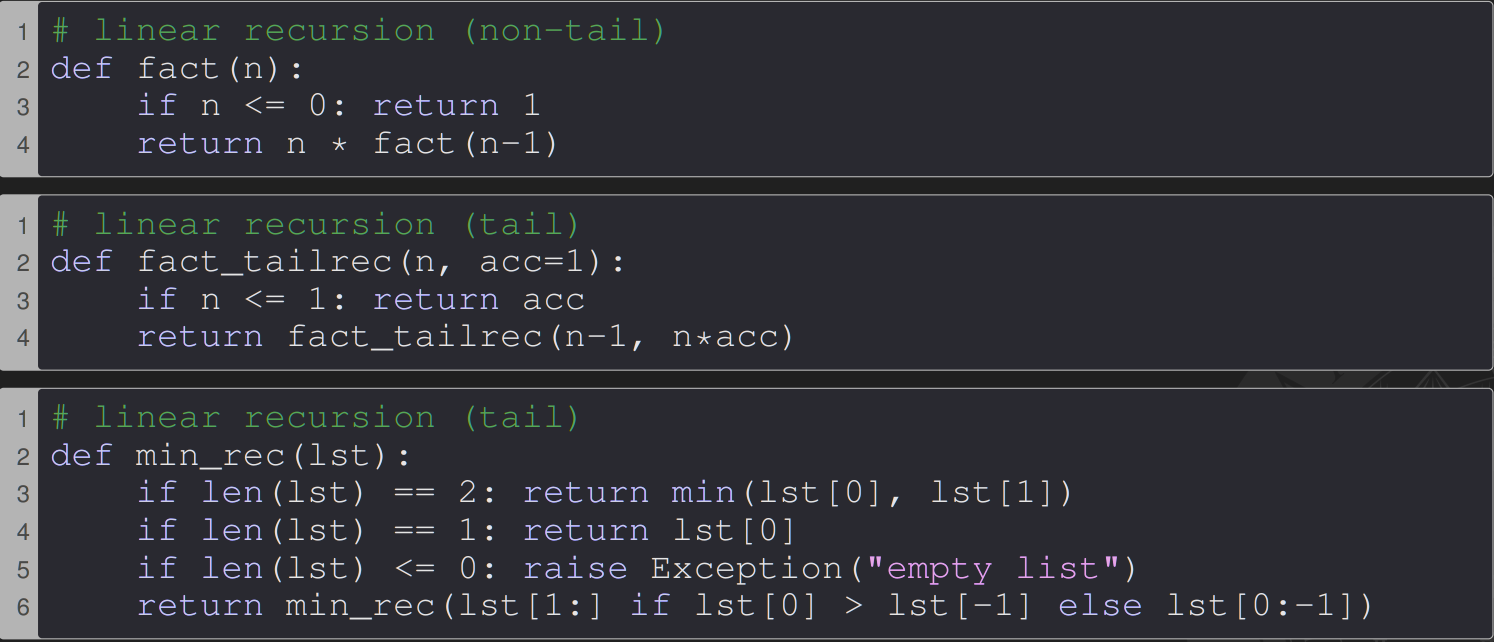
\includegraphics[keepaspectratio]{images/image222.png}}}

{}

{Multipla}

{\pandocbounded{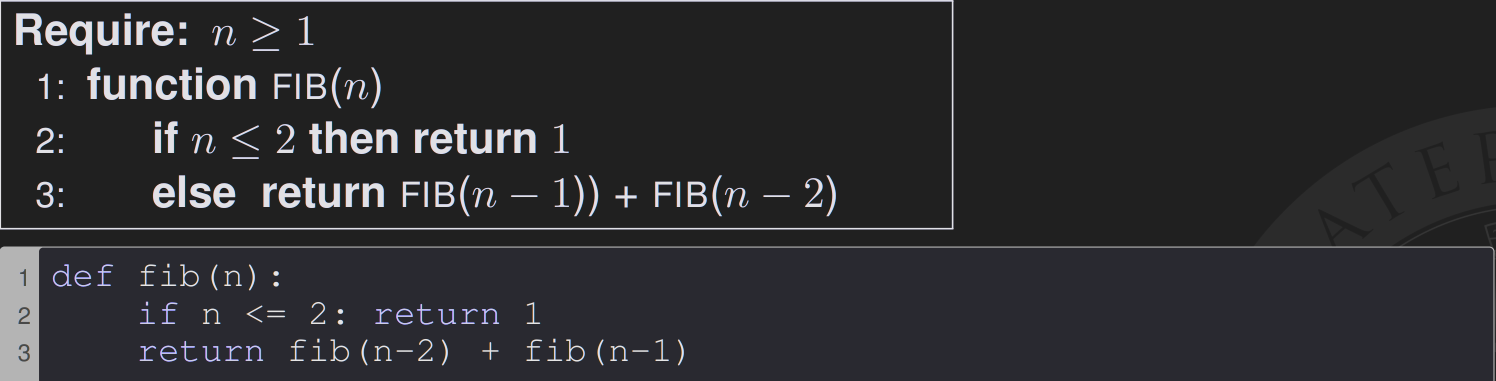
\includegraphics[keepaspectratio]{images/image257.png}}}

{}

{Mutua}

{\pandocbounded{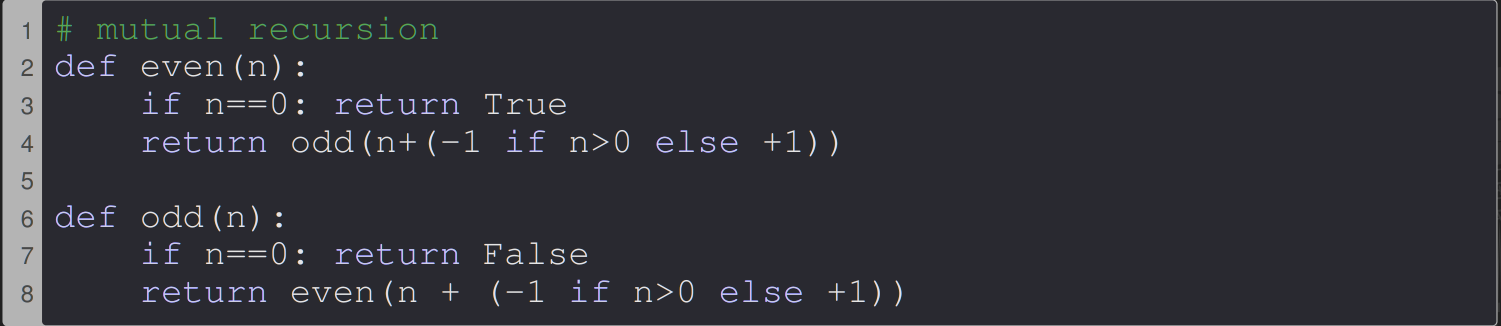
\includegraphics[keepaspectratio]{images/image261.png}}}

{}

{}

{Efficienza degli algoritmi}

{Caratterizzare l'efficienza è un aspetto importante dell'analisi e
progettazione di algoritmi, esistono due nozioni fondamentali:}

\begin{itemize}
\tightlist
\item
  {efficienza in tempo}
\item
  {efficienza in spazio}
\end{itemize}

\section{\texorpdfstring{{Tempi di
esecuzione}}{Tempi di esecuzione}}\label{h.wvdfqf8q2ihk}

{$\tau$  (Tau) è la funzione che serve per identificare il tempo di
esecuzione, determinata dalla natura e struttura dell'algoritmo.}

{La $\tau$  dipende dalla dimensione n dell'input, dalle istanze dell'input
(se dobbiamo valutare un algoritmo di ordinamento il modo in cui l'array
ci arriva è essenziale) e dall'esecutore.}

{In sostanza:}

{}

{`\,'}{La variazione del tempo d'esecuzione al variare della dimensione
n dell'input può essere caratterizzata da una funzione $\tau$  (n)}{`\,'}

{}

{Alcune forme frequenti di $\tau$ (n) sono:}

\begin{itemize}
\tightlist
\item
  {meno che
  lineare:}{~}\pandocbounded{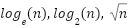
\includegraphics[keepaspectratio]{images/image1.png}}{~}{--\textgreater{}
  }{all'aumento di n il tempo di esecuzione aumenta lentamente}
\item
  {lineare}{:
  }\pandocbounded{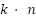
\includegraphics[keepaspectratio]{images/image2.png}}
\item
  {più che lineare}{:
  }\pandocbounded{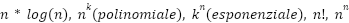
\includegraphics[keepaspectratio]{images/image3.png}}{~--\textgreater{}
  }{all'aumento di n il tempo di esecuzione aumenta velocemente}
\end{itemize}

{\pandocbounded{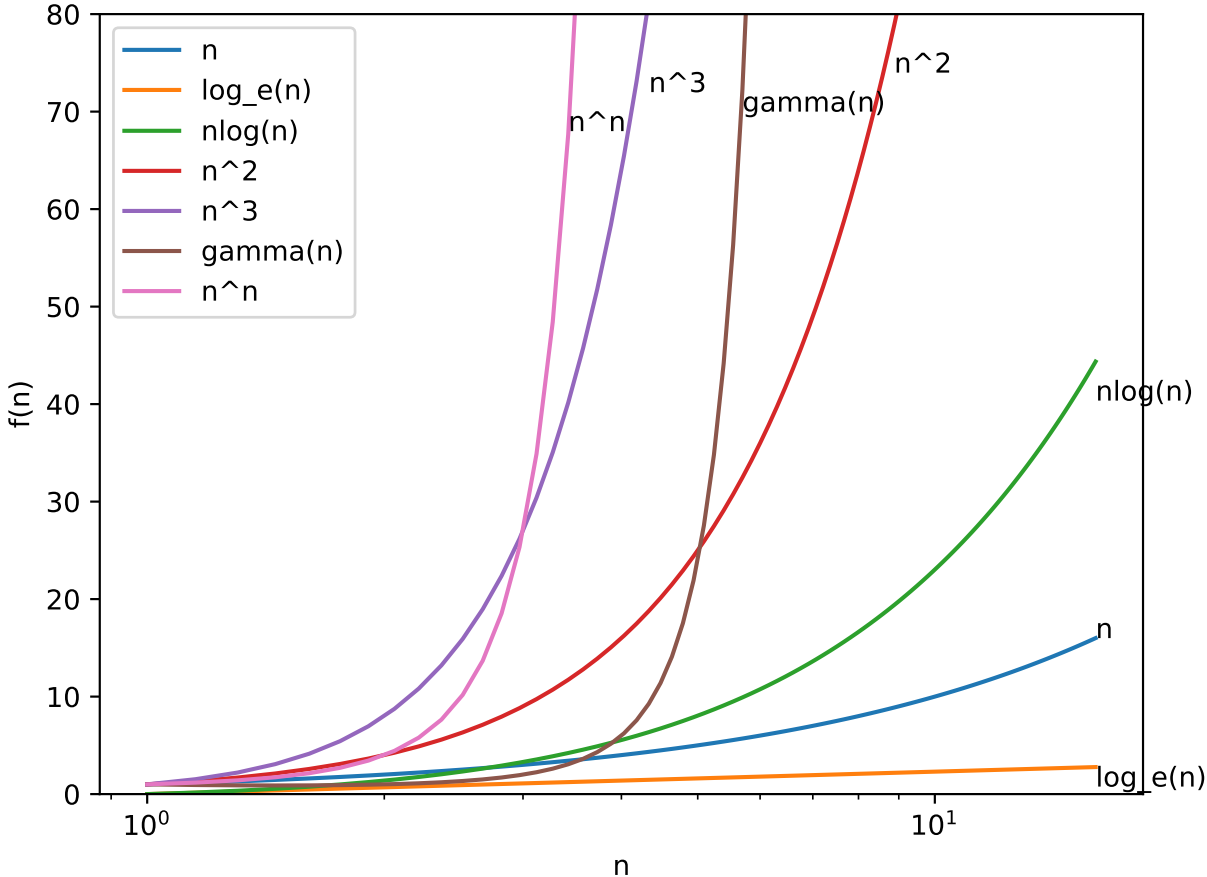
\includegraphics[keepaspectratio]{images/image252.png}}}

{Per una dimensione n esistono tre casi:}

\begin{enumerate}
\tightlist
\item
  {Best case}{: le configurazioni della struttura dati di ingresso
  }\pandocbounded{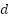
\includegraphics[keepaspectratio]{images/image4.png}}{~che
  danno luogo al tempo minimo;}
\item
  {Average case}{: le configurazioni della struttura dati di ingresso
  }\pandocbounded{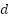
\includegraphics[keepaspectratio]{images/image4.png}}{~ritenute
  ``normali'' (e.g., più frequenti in pratica);}
\item
  {Worst case}{: le configurazioni della struttura dati di }{ingresso
  }\pandocbounded{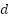
\includegraphics[keepaspectratio]{images/image4.png}}{~che}{~danno
  luogo al tempo massimo.}
\end{enumerate}

{}

{La prima casistica non è rilevante, invece:}

\begin{itemize}
\tightlist
\item
  {la }{complessità worst-case}{~serve per capire i limiti di
  applicabilità pratica permettendo di fare ragionamenti sulla safety
  (controlli real-time);}
\item
  {la }{complessità average-case}{~è difficile da valutare essendo non
  semplice caratterizzare input tipici.}
\end{itemize}

\section{\texorpdfstring{{Andamento
asintotico}}{Andamento asintotico}}\label{h.k8awz8fg85mc}

{Essendo che $\tau$ (n) è influenzato dal hardware o dal linguaggio di
programmazione si vuole }{astrarre}{~da questi aspetti, infatti non ci
interessa quanto tempo ci mette un determinato computer rispetto ad un
altro ma bisogna capire l'andamento del tempo asintoticamente quindi al
crescere dell'input.}

{Anche con tre tempi di esecuzione differenti (essendo fatti su hardware
diversi) essi potrebbero essere accomunati dallo stesso andamento.}

\section{\texorpdfstring{{Modello di
calcolo}}{Modello di calcolo}}\label{h.acnckxax5on2}

{Durante lo studio degli algoritmi si considera un modello di calcolo
standard chiamato }{RAM }{(Random Access Machine)}{, cioè un sistema
}{mono-processore}{~(istruzioni in sequenza) dove le istruzioni semplici
richiedono tempo costante.}

{Con
}\pandocbounded{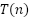
\includegraphics[keepaspectratio]{images/image5.png}}{~denotiamo
il tempo stimato per l'esecuzione dell'algoritmo nella RAM (stima tempo
effettivo $\tau$ (n)).}

\section{\texorpdfstring{{Complessità computazionale
}}{Complessità computazionale }}\label{h.iscgqksqr7yi}

{È l'ordine di grandezza della funzione T(n)}

{}

\section{\texorpdfstring{{Ordini di
infiniti}}{Ordini di infiniti}}\label{h.ejv96cbyxkh9}

{Una funzione
}\pandocbounded{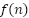
\includegraphics[keepaspectratio]{images/image6.png}}{~tale
che
}\pandocbounded{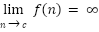
\includegraphics[keepaspectratio]{images/image7.png}}{~è
infinita per
}\pandocbounded{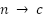
\includegraphics[keepaspectratio]{images/image8.png}}{.}

{Due funzioni
}\pandocbounded{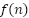
\includegraphics[keepaspectratio]{images/image6.png}}{~e
}\pandocbounded{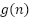
\includegraphics[keepaspectratio]{images/image9.png}}{~sono
}{infiniti simultanei}{~se entrambe sono infinite per
}\pandocbounded{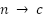
\includegraphics[keepaspectratio]{images/image8.png}}{.}

{}

{Quindi se abbiamo funzioni con dei tempi di esecuzione
}\pandocbounded{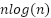
\includegraphics[keepaspectratio]{images/image10.png}}{~o
}\pandocbounded{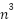
\includegraphics[keepaspectratio]{images/image11.png}}{~con
}\pandocbounded{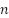
\includegraphics[keepaspectratio]{images/image12.png}}{~che
tende all'infinito avremo solo funzioni tendenti ad esso e non saremo in
grado di capire quale ha tempi di esecuzione migliori. Quindi per
confrontare diversi infiniti dobbiamo determinare quale ``}{tende
all\textquotesingle infinito più rapidamente}{'' andando a studiare il
limite del rapporto
}\pandocbounded{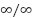
\includegraphics[keepaspectratio]{images/image13.png}}{~(forma
indeterminata).}

{Le casistiche sono:}

{\pandocbounded{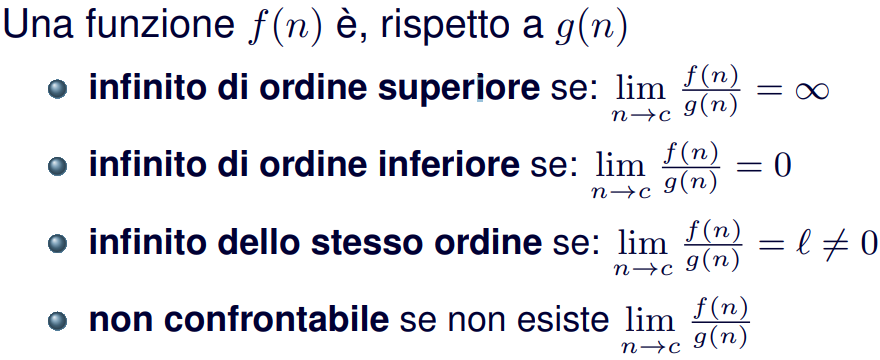
\includegraphics[keepaspectratio]{images/image251.png}}}

\section{\texorpdfstring{{Analisi
asintotica}}{Analisi asintotica}}\label{h.vqbdamxhmamw}

{Abbiamo capito che il tasso di crescita del tempo stimato di esecuzione
T(n) di un algoritmo da una semplice caratterizzazione della relativa
efficienza e calcolare il tempo esatto non serve visto che per input
grandi le costanti moltiplicative e i termini di ordine inferiore del
tempo effettivo di esecuzione sono trascurabili ed solo la forma della
funzione di n che definisce l'andamento.}

{}

{Efficienza asintotica \textbar{} Def: }

{È quella che si studia per dimensioni di n tali per cui solo l'ordine
del tasso di crescita è rilevante}

{Tempo di esecuzione asintotico \textbar{} Def: }

{Approssimazione del tempo d'esecuzione di un algoritmo mediante una
``più semplice'' funzione di simile ordine di crescita}

{\pandocbounded{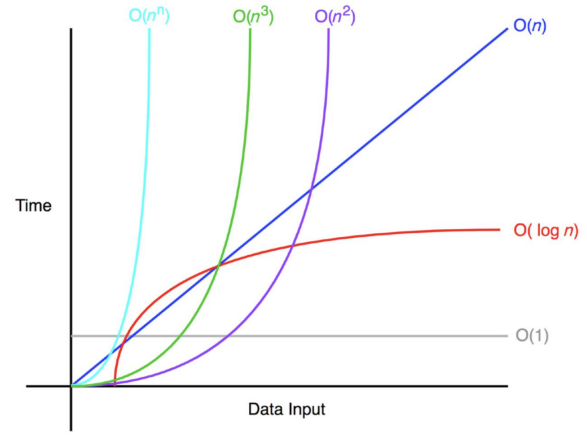
\includegraphics[keepaspectratio]{images/image243.png}}}

\subsection{\texorpdfstring{{Notazione
asintotica}}{Notazione asintotica}}\label{h.9566r1d59a7c}

{Notazione standard per caratterizzare l'efficienza in tempo di un
algoritmo}

{\pandocbounded{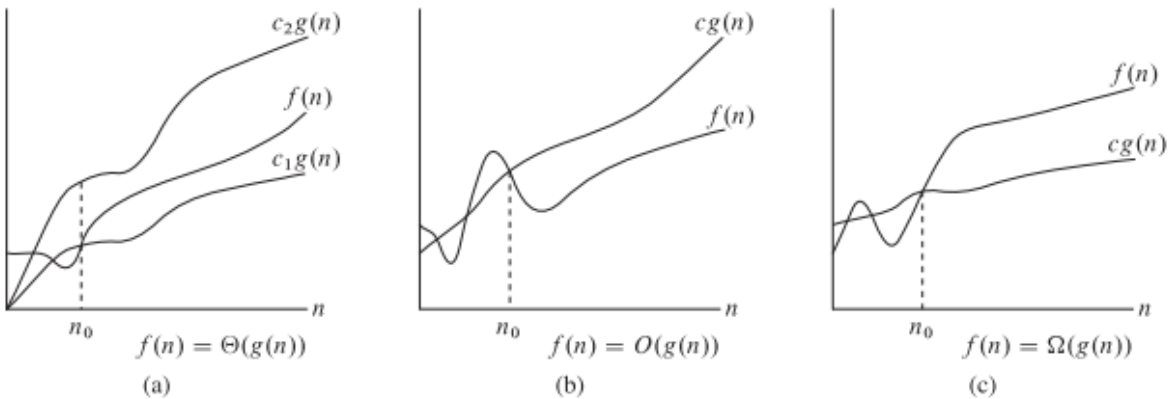
\includegraphics[keepaspectratio]{images/image225.png}}}

{Si suddividono in altre 3 notazioni che sono:}

{}

\begin{itemize}
\tightlist
\item
  \pandocbounded{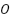
\includegraphics[keepaspectratio]{images/image14.png}}{~{[}O-grande{]}}{:
  data una funzione (di confronto)
  }\pandocbounded{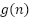
\includegraphics[keepaspectratio]{images/image9.png}}{:}
\end{itemize}

{~}\pandocbounded{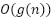
\includegraphics[keepaspectratio]{images/image15.png}}{~individua
tutte le funzioni
}\pandocbounded{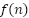
\includegraphics[keepaspectratio]{images/image6.png}}{~tale
per cui esiste una costante reale maggiore di 0
(}\pandocbounded{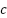
\includegraphics[keepaspectratio]{images/image16.png}}{,
}\pandocbounded{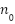
\includegraphics[keepaspectratio]{images/image17.png}}{)
tale per cui questa condizione è verificata:
}\pandocbounded{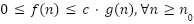
\includegraphics[keepaspectratio]{images/image18.png}}{~(}\pandocbounded{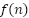
\includegraphics[keepaspectratio]{images/image6.png}}{~compresa
tra 0 e
}\pandocbounded{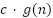
\includegraphics[keepaspectratio]{images/image19.png}}{~per
tutti i valori di
}\pandocbounded{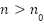
\includegraphics[keepaspectratio]{images/image20.png}}{).}

{Quindi possiamo individuare un certo valore
}\pandocbounded{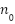
\includegraphics[keepaspectratio]{images/image17.png}}{~di
dimensioni del problema e una certa costante moltiplicativa tale per cui
dal punto
}\pandocbounded{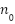
\includegraphics[keepaspectratio]{images/image17.png}}{~individuato,
la funzione
}\pandocbounded{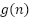
\includegraphics[keepaspectratio]{images/image9.png}}{~(moltiplicata
per un fattore a scelta) va a dominare dall'alto la nostra funzione.}

{In sostanza:}

\pandocbounded{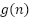
\includegraphics[keepaspectratio]{images/image9.png}}{~è
un limite superiore o upper bound asintotico per
}\pandocbounded{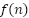
\includegraphics[keepaspectratio]{images/image6.png}}

{e}

\pandocbounded{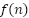
\includegraphics[keepaspectratio]{images/image6.png}}{~asintoticamente
cresce come o meno di
}\pandocbounded{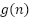
\includegraphics[keepaspectratio]{images/image9.png}}

{}

{Esempio:}

{Dimostrare che
}\pandocbounded{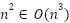
\includegraphics[keepaspectratio]{images/image21.png}}

{~ ~ ~ ~ ~ ~ ~ ~ ~ ~ ~ }{~
}\pandocbounded{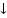
\includegraphics[keepaspectratio]{images/image22.png}}{~
~ ~ ~ ~
}\pandocbounded{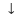
\includegraphics[keepaspectratio]{images/image23.png}}

{~ ~ ~ ~ ~ ~ ~ ~ ~ ~ ~ ~ ~
~}\pandocbounded{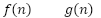
\includegraphics[keepaspectratio]{images/image24.png}}

{Dobbiamo usare la definizione di
}\pandocbounded{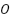
\includegraphics[keepaspectratio]{images/image14.png}}{,
}{quindi esiste una costante
}\pandocbounded{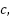
\includegraphics[keepaspectratio]{images/image25.png}}\pandocbounded{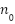
\includegraphics[keepaspectratio]{images/image17.png}}{~tale
per cui
}\pandocbounded{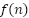
\includegraphics[keepaspectratio]{images/image6.png}}{~è
maggiorata da
}\pandocbounded{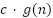
\includegraphics[keepaspectratio]{images/image19.png}}{~e
questa cosa è valida per ogni
}\pandocbounded{\includegraphics[keepaspectratio]{images/image26.png}}{.}

{Applichiamo la disequazione che la formula ci da:}

\pandocbounded{\includegraphics[keepaspectratio]{images/image27.png}}{~}\pandocbounded{\includegraphics[keepaspectratio]{images/image28.png}}{~}\pandocbounded{\includegraphics[keepaspectratio]{images/image29.png}}

{~ ~ ~ ~ ~ ~ ~ ~ ~ ~ ~ ~ ~
~}\pandocbounded{\includegraphics[keepaspectratio]{images/image30.png}}

{~ ~ ~ ~ ~ ~ ~ ~ ~ ~ ~ ~ ~ ~ ~ ~ ~ ~ ~ ~ ~ ~
~}\pandocbounded{\includegraphics[keepaspectratio]{images/image31.png}}{~
}\pandocbounded{\includegraphics[keepaspectratio]{images/image28.png}}{~}\pandocbounded{\includegraphics[keepaspectratio]{images/image32.png}}

{}

{}

\begin{itemize}
\tightlist
\item
  \pandocbounded{\includegraphics[keepaspectratio]{images/image33.png}}{~{[}Omega-grande{]}}{:
  data una funzione
  }\pandocbounded{\includegraphics[keepaspectratio]{images/image9.png}}{:}
\end{itemize}

\pandocbounded{\includegraphics[keepaspectratio]{images/image34.png}}{~individua
tutte le funzioni
}\pandocbounded{\includegraphics[keepaspectratio]{images/image6.png}}{~tale
per cui esiste una costante reale maggiore di 0
(}\pandocbounded{\includegraphics[keepaspectratio]{images/image16.png}}{,
}\pandocbounded{\includegraphics[keepaspectratio]{images/image17.png}}{)
tale per cui questa condizione è verificata:}

\pandocbounded{\includegraphics[keepaspectratio]{images/image35.png}}{~(}\pandocbounded{\includegraphics[keepaspectratio]{images/image9.png}}{~compresa
tra 0 e
}\pandocbounded{\includegraphics[keepaspectratio]{images/image6.png}}{~per
tutti i valori di
}\pandocbounded{\includegraphics[keepaspectratio]{images/image20.png}}{).}

{In sostanza:}

\pandocbounded{\includegraphics[keepaspectratio]{images/image9.png}}{~è
un limite inferiore o lower bound asintotico per
}\pandocbounded{\includegraphics[keepaspectratio]{images/image6.png}}

{e}

\pandocbounded{\includegraphics[keepaspectratio]{images/image6.png}}{~asintoticamente
cresce come o più di
}\pandocbounded{\includegraphics[keepaspectratio]{images/image9.png}}

{}

{}

{}

\begin{itemize}
\tightlist
\item
  \pandocbounded{\includegraphics[keepaspectratio]{images/image36.png}}{~{[}Theta-grande{]}}{:
  data una funzione
  }\pandocbounded{\includegraphics[keepaspectratio]{images/image9.png}}{:}
\end{itemize}

\pandocbounded{\includegraphics[keepaspectratio]{images/image37.png}}{~individua
tutte le funzioni
}\pandocbounded{\includegraphics[keepaspectratio]{images/image6.png}}{~tale
per cui esiste una costante reale maggiore di 0
(}\pandocbounded{\includegraphics[keepaspectratio]{images/image38.png}}{,}\pandocbounded{\includegraphics[keepaspectratio]{images/image39.png}}{,
}\pandocbounded{\includegraphics[keepaspectratio]{images/image17.png}}{)
tale per cui questa condizione è verificata: }

\pandocbounded{\includegraphics[keepaspectratio]{images/image40.png}}

{Quindi
}\pandocbounded{\includegraphics[keepaspectratio]{images/image6.png}}{~da
un certo punto in poi
(}\pandocbounded{\includegraphics[keepaspectratio]{images/image17.png}}{)
è compresa tra
}\pandocbounded{\includegraphics[keepaspectratio]{images/image41.png}}{~}{e
}\pandocbounded{\includegraphics[keepaspectratio]{images/image42.png}}

{In sostanza:}

\pandocbounded{\includegraphics[keepaspectratio]{images/image9.png}}{~è
un limite asintotico stretto o tight bound per
}\pandocbounded{\includegraphics[keepaspectratio]{images/image6.png}}

{e}

\pandocbounded{\includegraphics[keepaspectratio]{images/image9.png}}{~e
}\pandocbounded{\includegraphics[keepaspectratio]{images/image6.png}}{~hanno
lo stesso ordine di grandezza}

{}

{}

{NB}{: }{se
}\pandocbounded{\includegraphics[keepaspectratio]{images/image6.png}}{~appartiene
a }{O-grande}{~di
}\pandocbounded{\includegraphics[keepaspectratio]{images/image43.png}}{~allora
sicuramente apparterrà anche a
}{O-grande}{~}\pandocbounded{\includegraphics[keepaspectratio]{images/image11.png}}{,
}{se invece
}\pandocbounded{\includegraphics[keepaspectratio]{images/image6.png}}{~appartiene
a }{Theta-grande}{~di
}\pandocbounded{\includegraphics[keepaspectratio]{images/image43.png}}{~sicuramente
}{non }{apparterrà ne a ~}{Theta-grande}{~di
}\pandocbounded{\includegraphics[keepaspectratio]{images/image12.png}}{~ne
a ~}{Theta-grande}{~di
}\pandocbounded{\includegraphics[keepaspectratio]{images/image11.png}}{~.}

{}

\subsubsection{\texorpdfstring{{Proprietà e
osservazioni}}{Proprietà e osservazioni}}\label{h.m9cfkuaj2xoy}

\begin{itemize}
\tightlist
\item
  {Relazioni}{: una funzione
  }\pandocbounded{\includegraphics[keepaspectratio]{images/image44.png}}{~appartiene
  a
  }\pandocbounded{\includegraphics[keepaspectratio]{images/image45.png}}{)
  se solo se la funzione appartiene anche a
  }\pandocbounded{\includegraphics[keepaspectratio]{images/image15.png}}{~e
  }\pandocbounded{\includegraphics[keepaspectratio]{images/image34.png}}{;}
\item
  {Regola della somma:}{~se una funzione
  }\pandocbounded{\includegraphics[keepaspectratio]{images/image5.png}}{~appartiene
  a
  }\pandocbounded{\includegraphics[keepaspectratio]{images/image46.png}}{~allora
  possiamo semplificare considerando Theta-grande come il massimo delle
  due funzioni
  {[}}\pandocbounded{\includegraphics[keepaspectratio]{images/image47.png}}{{]};}
\item
  {I termini di grado inferiore non interessano}{: se abbiamo
  }\pandocbounded{\includegraphics[keepaspectratio]{images/image48.png}}{~}{ci
  interessa}{~valutare solo quello con il grado maggiore, essendo gli
  altri ``contenuti'' in esso;}
\end{itemize}

\section{\texorpdfstring{{Complessità
costrutti}}{Complessità costrutti}}\label{h.un2ps9tq1l7k}

{Per ogni costrutto semplice abbiamo le seguenti complessità:}

\begin{itemize}
\tightlist
\item
  {Istruzioni semplici}{: }{qui ci sono assegnamenti e operazioni
  aritmetiche/logiche/relazionali; tutti hanno
  }\pandocbounded{\includegraphics[keepaspectratio]{images/image49.png}}{.}
\item
  {Sequenza di istruzioni semplici}{: uguale a sopra
  (}\pandocbounded{\includegraphics[keepaspectratio]{images/image49.png}}{).}
\item
  {Costrutti selettivi}{: con condizione pari a
  }\pandocbounded{\includegraphics[keepaspectratio]{images/image49.png}}{:}
\end{itemize}

\begin{itemize}
\tightlist
\item
  \pandocbounded{\includegraphics[keepaspectratio]{images/image50.png}}{;}
\item
  \pandocbounded{\includegraphics[keepaspectratio]{images/image51.png}}{;}
\item
  {Caso peggiore:
  }\pandocbounded{\includegraphics[keepaspectratio]{images/image52.png}}{;}
\item
  {Caso maggiore:
  }\pandocbounded{\includegraphics[keepaspectratio]{images/image53.png}}{.}
\end{itemize}

\begin{itemize}
\tightlist
\item
  {Costrutti iterativi}{: }
\end{itemize}

\begin{itemize}
\tightlist
\item
  {for}{~per
  }\pandocbounded{\includegraphics[keepaspectratio]{images/image54.png}}{~iterazioni
  e contando che
  }\pandocbounded{\includegraphics[keepaspectratio]{images/image55.png}}
\end{itemize}

\begin{itemize}
\tightlist
\item
  \pandocbounded{\includegraphics[keepaspectratio]{images/image56.png}}{;}
\item
  \pandocbounded{\includegraphics[keepaspectratio]{images/image57.png}}{;}
\item
  {Caso peggiore:
  }\pandocbounded{\includegraphics[keepaspectratio]{images/image58.png}}{;}
\item
  {Caso maggiore:
  }\pandocbounded{\includegraphics[keepaspectratio]{images/image59.png}}{.}
\end{itemize}

\begin{itemize}
\tightlist
\item
  {while}{~e in funzione del numero min e max di iterazioni
  (}\pandocbounded{\includegraphics[keepaspectratio]{images/image60.png}}{,}\pandocbounded{\includegraphics[keepaspectratio]{images/image61.png}}{)}
\end{itemize}

\begin{itemize}
\tightlist
\item
  \pandocbounded{\includegraphics[keepaspectratio]{images/image62.png}}{~e
  }\pandocbounded{\includegraphics[keepaspectratio]{images/image63.png}}{;}
\item
  {Caso peggiore:
  }\pandocbounded{\includegraphics[keepaspectratio]{images/image64.png}}{;}
\item
  {Caso maggiore:
  }\pandocbounded{\includegraphics[keepaspectratio]{images/image65.png}}{.}
\end{itemize}

\subsection{\texorpdfstring{{Esempio}}{Esempio}}\label{h.x799yxcvntk0}

{\pandocbounded{\includegraphics[keepaspectratio]{images/image219.png}}}

{}

{Ricorrenze}

{Il modo di calcolare la complessità degli algoritmi visto
precedentemente non è applicabile alle funzioni ricorsive, infatti per
calcolare la complessità, dobbiamo considerare anche il costo della
chiamata ricorsiva andando a ottenere }{equazioni ricorrenti}{.}

{}

{Ora distinguiamo due contributi:}

\begin{itemize}
\tightlist
\item
  \pandocbounded{\includegraphics[keepaspectratio]{images/image6.png}}{:
  tempo di tutte le istruzioni che }{non }{contengono}{~chiamate
  ricorsive;}
\item
  \pandocbounded{\includegraphics[keepaspectratio]{images/image66.png}}{:
  tempo derivante dalle chiamate ricorsive, invocate su k \textless{} n
  (istanze più piccole del problema---cf. divide-et-impera).}
\end{itemize}

{}

\section{\texorpdfstring{{Metodi di risoluzione delle
ricorrenze}}{Metodi di risoluzione delle ricorrenze}}\label{h.dt5t05khniu5}

{Esistono tre metodi principali:}

\begin{enumerate}
\tightlist
\item
  {Metodo iterativo:}{~si espande l'equazione fino ad arrivare a una
  espressione in funzione di
  }\pandocbounded{\includegraphics[keepaspectratio]{images/image12.png}}{~e
  costanti;}
\end{enumerate}

{\pandocbounded{\includegraphics[keepaspectratio]{images/image199.png}}}

{\pandocbounded{\includegraphics[keepaspectratio]{images/image205.png}}}

\begin{enumerate}
\setcounter{enumi}{1}
\tightlist
\item
  {~Metodo della sostituzione}{: in questo caso:
  }\pandocbounded{\includegraphics[keepaspectratio]{images/image5.png}}{~appartiene
  a
  }\pandocbounded{\includegraphics[keepaspectratio]{images/image67.png}}{~quindi
  si effettua un ``guess'' sulla possibile soluzione e si utilizza
  l'induzione matematica per dimostrare la correttezza della soluzione;}
\end{enumerate}

{\pandocbounded{\includegraphics[keepaspectratio]{images/image201.png}}}

\begin{enumerate}
\setcounter{enumi}{2}
\tightlist
\item
  {Metodo dell'esperto}{: basato sul Master Theorem, per algoritmi della
  forma T(n) = aT(n/b) + f(n) (divide-et-impera).}
\end{enumerate}

{}

\subsection{\texorpdfstring{{Esempi}}{Esempi}}\label{h.mvrj1crn0xfl}

{\pandocbounded{\includegraphics[keepaspectratio]{images/image238.png}}}

{}

{Problema della ricerca}

{In molte applicazioni è necessario ricercare un elemento all'interno di
una struttura dati senza saperne la posizione, o non
}{potendovi}{~accedere direttamente.}

{}

{La formulazione del problema della ricerca si basa su:}

\begin{itemize}
\tightlist
\item
  {modalità di accesso}{~(casuale,sequenziale,...);}
\item
  {rappresentazione della posizione dell'elemento}{~(es. indice,
  puntatore, ...);}
\item
  {rappresentazione della proprietà dell'elemento}{~(es. valore,
  predicato sul valore, posizione...);}
\end{itemize}

{}

{Usando un accesso di tipo }{casuale }{l'}{accesso}{~}{ad un elemento
è}{~}{costante}{~}{indipendentemente dall posizione
{[}}\pandocbounded{\includegraphics[keepaspectratio]{images/image49.png}}{{]}
invece usando l'accesso }{sequenziale }{tutto }{dipende dalla
distanza}{~tra l'elemento desiderato e l'ultimo elemento acceduto (tra
}\pandocbounded{\includegraphics[keepaspectratio]{images/image68.png}}{~e
}\pandocbounded{\includegraphics[keepaspectratio]{images/image69.png}}{~è
}\pandocbounded{\includegraphics[keepaspectratio]{images/image70.png}}{.}

{}

{Negli esempi successivi si userà un }{array}{~quindi una struttura dati
con le seguenti proprietà:}

\begin{itemize}
\tightlist
\item
  {modalità d'accesso}{: accesso casuale;}
\item
  {rappresentazione posizione}{: attraverso indice}
\item
  {rappresentazione proprietà}{: mediante una nozione di uguaglianza
  }{equal}{~che deve essere:}
\end{itemize}

\begin{itemize}
\tightlist
\item
  {riflessiva}{: }{equal(a,a)}{;}
\item
  {simmetrica}{: }{equal(a,b)
  }\pandocbounded{\includegraphics[keepaspectratio]{images/image28.png}}{~equal(b,a)}{;}
\item
  {transitica}{: }{equal(a,b)
  }\pandocbounded{\includegraphics[keepaspectratio]{images/image71.png}}{~equal(b,c)
  }\pandocbounded{\includegraphics[keepaspectratio]{images/image28.png}}{~equal(a,c)}{.}
\end{itemize}

{}

{}

{Def \textbar{} Ricerca su sequenza }{indicizzata}{~}

{Data una sequenza }{indicizzata}{~di elementi
}\pandocbounded{\includegraphics[keepaspectratio]{images/image72.png}}{~e
un valore
}\pandocbounded{\includegraphics[keepaspectratio]{images/image73.png}}{~da
ricercare, si vuole trovare un indice i tale che
}{equal}{(}\pandocbounded{\includegraphics[keepaspectratio]{images/image74.png}}{)
è vera. }

\section{\texorpdfstring{{Tipi di
ricerca}}{Tipi di ricerca}}\label{h.rq59z6qkkgr}

\subsection{\texorpdfstring{{Lineare}}{Lineare}}\label{h.z3vimw7ty6l9}

{l'idea è quella di esaminare in sequenza tutti gli elementi della
struttura dati, confrontandoli con l'elemento desiderato:}

{\pandocbounded{\includegraphics[keepaspectratio]{images/image240.png}}}

{Questo algoritmo ha una crescita lineare nel caso medio/peggiore, per
quanto riguarda l'analisi della complessità:}

\begin{itemize}
\tightlist
\item
  {Caso migliore}{:
  }\pandocbounded{\includegraphics[keepaspectratio]{images/image75.png}}
\item
  {Caso peggiore}{:
  }\pandocbounded{\includegraphics[keepaspectratio]{images/image76.png}}
\item
  {Caso medio}{:
  }\pandocbounded{\includegraphics[keepaspectratio]{images/image77.png}}
\end{itemize}

\subsubsection{\texorpdfstring{{Minimo/massimo}}{Minimo/massimo}}\label{h.z2y10qkdgb72}

{Adattando l'algoritmo precedente, in quanto la proprietà non è più
verificabile in modo indipendente per ogni elemento, possiamo fare una
ricerca del minimo/massimo in una lista non ordinata di numeri; l'idea
dietro è quella di tenere traccia del risultato parziale.}

{\pandocbounded{\includegraphics[keepaspectratio]{images/image224.png}}}

{Per qualunque coppia di oggetti }{x e y}{~dev'essere definita una
relazione Booleana better (x, y) che dice se x dev'essere preferito a y
}

\subsection{\texorpdfstring{{Binaria}}{Binaria}}\label{h.bg4jjz5xisrc}

{in alcuni casi la struttura dati d'ingresso può essere già ordinata,
quindi possiamo assumere che gli elementi dell'array siano ordinati
rispetto a una relazione d'ordine }{less}{, dove il primo elemento è
minore rispetto al successivo, o }{equal}{~dove due elementi adiacenti
sono uguali.}

{Utile per il gioco guess a number o un dizionario}

{}

{In questo algoritmo per trovare un numero all'interno della struttura
dati (ordinata) servirà tenere traccia della porzione dell'array da
esaminare usando due indici, }{from}{~e }{to}{, che tengono traccia del
primo e ultimo elemento utile. In questo modo si andrà a scartare la
porzione di array che non ci interessa.}

{}

{Ad ogni iterazione scegliamo un elemento utile, detto
}{pivot}{~(}\pandocbounded{\includegraphics[keepaspectratio]{images/image78.png}}{),
contenuto fra from e to, verifichiamo se il pivot è l'elemento da
ricercare, se }{sì}{~terminiamo altrimenti restringiamo il campo:}

\begin{itemize}
\tightlist
\item
  {less(elem,
  }\pandocbounded{\includegraphics[keepaspectratio]{images/image78.png}}{)}{:
  poniamo to = m - 1;}
\item
  {¬less(elem,}\pandocbounded{\includegraphics[keepaspectratio]{images/image79.png}}{)}{:
  poniamo from = m + 1.}
\end{itemize}

{}

{Dobbiamo anche considerare che, se l'elemento desiderato non è
contenuto nell'array, la riduzione della porzione da esaminare si
ridurrà all'insieme vuoto.}

{E per scegliere un elemento utile nella porzione }{from..to}{~conviene
usare la seguente formula: }{(from + to)/2 = from/2 + to/2}{.}

{}

{Visualizzazione del procedimento}

{\pandocbounded{\includegraphics[keepaspectratio]{images/image189.png}}}

{}

{L'algoritmo in pseudocodice è il seguente:}

{\pandocbounded{\includegraphics[keepaspectratio]{images/image262.png}}}

{L'analisi della complessità denota che nel caso generale
}\pandocbounded{\includegraphics[keepaspectratio]{images/image80.png}}{~e
nel migliore
}\pandocbounded{\includegraphics[keepaspectratio]{images/image81.png}}{.
Il caso peggiore è quando l'elemento non viene trovato quindi
}\pandocbounded{\includegraphics[keepaspectratio]{images/image82.png}}{~con
una crescita logaritmica.}

\section{\texorpdfstring{{Per interpolazione /
}{Interpolation}{~search}}{Per interpolazione / Interpolation~search}}\label{h.kzaw6w94yuiu}

{La ricerca per interpolazione è una variante migliorata della ricerca
binaria, che si basa sull'interpolazione }{{[}metodo per individuare
nuovi punti del piano cartesiano a partire da set finito di punti
dati{]}}{.}

{In questo algoritmo, per cercare di indovinare dove sarà l'elemento da
ricercare, si usa la formula:}

\pandocbounded{\includegraphics[keepaspectratio]{images/image83.png}}

{}

{Dove:}

\begin{itemize}
\tightlist
\item
  {Gli indici da considerare sono quelli dell'intervallo
  {[}}\pandocbounded{\includegraphics[keepaspectratio]{images/image84.png}}{,
  }\pandocbounded{\includegraphics[keepaspectratio]{images/image85.png}}{{]}}
\item
  {La formula offre una ``stima'' di dove è plausibile si possa trovare
  il target da trovare considerando:}
\end{itemize}

\begin{itemize}
\tightlist
\item
  \pandocbounded{\includegraphics[keepaspectratio]{images/image86.png}}{:
  la grandezza dell'intervallo considerato;}
\item
  \pandocbounded{\includegraphics[keepaspectratio]{images/image87.png}}{:
  ~la differenza tra il target da trovare e il più piccolo esaminato;}
\item
  \pandocbounded{\includegraphics[keepaspectratio]{images/image88.png}}{:
  la differenza tra il più grande e il più piccolo nell'intervallo
  esaminato;}
\end{itemize}

{}

{}

{Esempio di esecuzione {[}caso sfortunato{]}}

{\pandocbounded{\includegraphics[keepaspectratio]{images/image220.png}}}

{}

{}

{}

{}

{L'algoritmo in pseudocodice è il seguente:}

{\pandocbounded{\includegraphics[keepaspectratio]{images/image197.png}}}

{Per quanto riguarda l'analisi della complessità:}

\begin{itemize}
\tightlist
\item
  {Caso migliore}{:
  }\pandocbounded{\includegraphics[keepaspectratio]{images/image89.png}}
\item
  {Caso medio}{:
  }\pandocbounded{\includegraphics[keepaspectratio]{images/image90.png}}
\item
  {Caso peggiore}{:
  }\pandocbounded{\includegraphics[keepaspectratio]{images/image91.png}}
\end{itemize}

{}

{Strutture dati di base}

\section{\texorpdfstring{{Array
dinamici}}{Array dinamici}}\label{h.1smvnpk2qxek}

{Si superano i problemi degli array classici come l'impossibilità di
modificarlo a run-time o operazioni simili che hanno complessità
}\pandocbounded{\includegraphics[keepaspectratio]{images/image92.png}}{.}

{}

{L'allocazione ~in memoria può essere:}

\begin{itemize}
\tightlist
\item
  {Statica}{: il ciclo di vita del programma e dell'oggetto è uguale
  (creati/distrutti insieme);}
\item
  {Automatica}{: ~l'oggetto viene de/allocato automaticamente
  all'uscita/entrata di un contesto;}
\item
  {Dinamica}{: l'oggetto viene allocato e }{deallocato}{~su richiesta
  (malloc, free).}
\end{itemize}

{In maniera simile una }{struttura dati è}{~}{statica }{se ha
}{dimensione fissa}{~o }{dinamica }{se }{varia a run time}{.}

{}

{Recap C:}

{\pandocbounded{\includegraphics[keepaspectratio]{images/image203.png}}}

{}

{In linguaggi nuovi come Python gli array dinamici sono già presenti
sotto forma di liste, in C questo non è vero.}

{Per realizzarle abbiamo bisogno di funzioni per gestire dinamicamente
la memoria, la cosiddetta }{riallocazione}{, e tenere traccia della
dimensione corrente. }

{}

{La riallocazione è un'operazione costosa
(}\pandocbounded{\includegraphics[keepaspectratio]{images/image92.png}}{)
e quindi evitiamo di farla ogni cambio di dimensione, a questo punto
distinguiamo tra:}

\begin{itemize}
\tightlist
\item
  {Capacità}{: numero max di elementi contenuti;}
\item
  {Dimensione/Lunghezza}{: numero di elementi correnti all'interno della
  struttura dati.}
\end{itemize}

{\pandocbounded{\includegraphics[keepaspectratio]{images/image213.png}}}

{}

{Per lavorare sulle due variabili distinguiamo fra:}

\begin{itemize}
\tightlist
\item
  {Ridimensionamento}{: lavora sulla size;}
\item
  {Riallocazione}{: lavora sulla capacity, operazione che viene fatta
  meno di frequente e solo quando la size è piena.}
\end{itemize}

{Se abbiamo una }{espansione}{~vuol dire che:
}\pandocbounded{\includegraphics[keepaspectratio]{images/image93.png}}{,
ma c'è bisogno di ridimensionare con riallocazione solo se:
}\pandocbounded{\includegraphics[keepaspectratio]{images/image94.png}}{.
Con una }{contrazione }{invece abbiamo che:
}\pandocbounded{\includegraphics[keepaspectratio]{images/image95.png}}{~e
la riallocazione è necessaria.}

{Ora però dobbiamo capire quanta capacità supplementare va allocata o
tollerata in queste due fasi.}

\subsection{\texorpdfstring{{Ridimensionamento con espansione
lineare}}{Ridimensionamento con espansione lineare}}\label{h.h6ue9oz0kdt3}

{Distinguiamo in riallocazione e contrazione:}

\begin{itemize}
\tightlist
\item
  {in caso di necessità di }{riallocazione
  }{(}\pandocbounded{\includegraphics[keepaspectratio]{images/image94.png}}{),
  riserviamo un numero fisso di elementi in più
  }\pandocbounded{\includegraphics[keepaspectratio]{images/image96.png}}{~rispetto
  alla dimensione richiesta:}
\end{itemize}

\pandocbounded{\includegraphics[keepaspectratio]{images/image97.png}}

{}

\begin{itemize}
\tightlist
\item
  {in caso di contrazione, riduciamo la capacità solo se la differenza
  tra la capacità attuale e la nuova lunghezza richiesta supera una
  soglia
  }\pandocbounded{\includegraphics[keepaspectratio]{images/image98.png}}{:}
\end{itemize}

\pandocbounded{\includegraphics[keepaspectratio]{images/image99.png}}

{Ricordarsi di controllare che
}\pandocbounded{\includegraphics[keepaspectratio]{images/image100.png}}\pandocbounded{\includegraphics[keepaspectratio]{images/image98.png}}

{\pandocbounded{\includegraphics[keepaspectratio]{images/image194.png}}}

\subsection{\texorpdfstring{{Ridimensionamento con espansione
geometrica}}{Ridimensionamento con espansione geometrica}}\label{h.jvs3vttw93vb}

{In questo caso invece di usare una capacità supplementare fissa
}\pandocbounded{\includegraphics[keepaspectratio]{images/image96.png}}{~si
usa una capacità supplementare che è proporzionale alla lunghezza
richiesta
}\pandocbounded{\includegraphics[keepaspectratio]{images/image101.png}}{~di
un fattore
}\pandocbounded{\includegraphics[keepaspectratio]{images/image102.png}}{.}

{}

{In caso di contrazione riduciamo la capacità quando:
}\pandocbounded{\includegraphics[keepaspectratio]{images/image103.png}}{,
quindi i possibili frangenti sono:}

\begin{enumerate}
\tightlist
\item
  {Se
  }\pandocbounded{\includegraphics[keepaspectratio]{images/image104.png}}{~allora
  }\pandocbounded{\includegraphics[keepaspectratio]{images/image105.png}}
\item
  {Se
  }\pandocbounded{\includegraphics[keepaspectratio]{images/image106.png}}{~}{e
  con
  }\pandocbounded{\includegraphics[keepaspectratio]{images/image107.png}}{~allora
  }\pandocbounded{\includegraphics[keepaspectratio]{images/image105.png}}
\item
  {nessuna riallocazione}
\end{enumerate}

{\pandocbounded{\includegraphics[keepaspectratio]{images/image245.png}}}

\subsection{\texorpdfstring{{Complessità}}{Complessità}}\label{h.s1ly2x73jpem}

{\pandocbounded{\includegraphics[keepaspectratio]{images/image275.png}}}{\pandocbounded{\includegraphics[keepaspectratio]{images/image228.png}}}{\pandocbounded{\includegraphics[keepaspectratio]{images/image198.png}}}

\section{\texorpdfstring{{Pile /
Stack}}{Pile / Stack}}\label{h.xjbwfhafeawp}

{Struttura dati con accesso di tipo LIFO, l'ultimo elemento che entra è
il primo ad uscire. Le operazioni possibili sono:}

\begin{itemize}
\tightlist
\item
  {create}{~}{e }{destroy}{;}
\item
  {push}{: metti in cima;}
\item
  {pop}{: togli dalla cima;}
\item
  {top}{: vedi cosa c'è in cima;}
\item
  {isempty}{~e }{isfull}{: controllo vuota/piena.}
\end{itemize}

{}

{Per implementare una pila è sufficiente tenere traccia del numero di
elementi presenti e da questo dato si ricava anche la posizione di
inserimento o prelievo. L'implementazione risulta facile tramite array
(statico o dinamico):}

{\pandocbounded{\includegraphics[keepaspectratio]{images/image237.png}}}

{Dove }{n}{~tiene traccia del numero di elementi e allo stesso tempo
della prossima posizione di inserimento}

\section{\texorpdfstring{{Code /
Queue}}{Code / Queue}}\label{h.7jhc8mivm8lm}

{Struttura dati con modalità di accesso FIFO, ~il primo elemento che
entra è il primo ad uscire.}

{Utile se vogliamo processare una sequenza di richieste in base
all\textquotesingle ordine di arrivo e con un'attesa non infinita,
possiamo usare i }{buffer}{~se o il tasso di arrivo di richieste
(producer speed) non corrisponde alla capacità di
}{soddisfarle}{~(consumer speed)o il tasso di arrivo di richieste
(producer speed) non corrisponde alla capacità di
}{soddisfarle}{~(consumer speed).}

{}

{Le operazioni possibili sono:}

\begin{itemize}
\tightlist
\item
  {create}{~}{e }{destroy}{;}
\item
  {add}{~o }{enqueue}{: metti in coda o accodamento;}
\item
  {remove}{~o }{~dequeue}{: togli dalla coda;}
\item
  {front}{: vedi cosa c'è in cima (1° elemento);}
\item
  {isempty}{~e }{isfull}{: controllo vuota/piena.}
\end{itemize}

{}

{Per implementare una coda è sufficiente tenere traccia del numero di
elementi presenti e da questo dato si ricava anche la posizione di
inserimento o prelievo. }

{Tenendo traccia della testa
(}\pandocbounded{\includegraphics[keepaspectratio]{images/image44.png}}{),
il prelievo si attua semplicemente con lo spostamento in avanti di
}\pandocbounded{\includegraphics[keepaspectratio]{images/image44.png}}{.}

{}

{Si può sempre usare un array statico o dinamico e }{per evitare
problemi di complessità}{~la soluzione è implementare una }{coda
circolare}{~}{dove }{l'array viene interpretato come struttura
ciclica}{~(dove la posizione successiva all'ultima è quella di indice 0)
e per incrementare gli indici è comodo usare la capacity:}

{}

{Enqueue:
}\pandocbounded{\includegraphics[keepaspectratio]{images/image108.png}}{~\textbar{}
Dequeue:
}\pandocbounded{\includegraphics[keepaspectratio]{images/image109.png}}

{\pandocbounded{\includegraphics[keepaspectratio]{images/image256.png}}}

{Liste dinamiche}

{Utili per rappresentare collezioni di elementi organizzati linearmente
e per lavorare con collezioni che consentano di svolgere in modo
efficiente le operazioni di ricerca, inserimento, e cancellazione.}

{}

{Def \textbar{} Lista}{: }{struttura dati che immagazzina un insieme di
elementi in ordine }

{}

{Esistono diversi tipi di liste:}

\begin{itemize}
\tightlist
\item
  {Linked list}{: formata da nodi, ogni nodo contiene l'informazione e
  il riferimento all'elemento successivo.}
\end{itemize}

{\pandocbounded{\includegraphics[keepaspectratio]{images/image215.png}}}

{L'ordine degli elementi è dato dai collegamenti esistenti fra gli
elementi e non dal piazzamento in memoria, il primo elemento è la
}{testa}{~e l'ultimo è la }{coda}{.}

\begin{itemize}
\tightlist
\item
  {Doubly-linked list}{: ogni nodo contiene anche un collegamento
  all'elemento precedente; tipicamente sono noti sia il riferimento alla
  testa sia il riferimento alla coda.}
\end{itemize}

{\pandocbounded{\includegraphics[keepaspectratio]{images/image269.png}}}

\begin{itemize}
\tightlist
\item
  {Circular list}{: una linked list dove l'elemento in coda è collegato
  all'elemento in testa, il collegamento può essere singolo o doppio.}
\end{itemize}

{\pandocbounded{\includegraphics[keepaspectratio]{images/image230.png}}}

{}

{}

{Possiamo distinguere tre nozioni di ordinamento nelle liste:}

\begin{enumerate}
\tightlist
\item
  {Ordine strutturale:}{~ l'ordine risultante dai collegamenti fra i
  nodi;}
\item
  {Ordine logico:}{~ l'ordine esistente tra gli elementi sulla base di
  una relazione d'ordine;}
\item
  {Ordine fisico}{: ~l'ordine degli elementi in memoria.}
\end{enumerate}

{}

{Def \textbar{} Lista ordinata}{: }{una lista dove l'ordine strutturale
corrisponde all'ordine logico}

\section{\texorpdfstring{{Implementazione}}{Implementazione}}\label{h.uwpmwwnk9p6k}

{L'implementazione può avvenire su array statici o dinamici dove ogni
elemento dell'array è un nodo della lista e il collegamento è dato
dall'indice dell'elemento successivo. Con gli array statici c'è il
problema di quanta memoria allocare e nei dinamici della rimozione dei
nodi e della frammentazione della memoria contigua associata all'array
dinamico.}

{}

{Normalmente l'implementazione avviene tramite allocazione dinamica dei
nodi, si definisce la lista come struttura dati ricorsivamente
definita:}

{\pandocbounded{\includegraphics[keepaspectratio]{images/image270.png}}}

{Una }{list}{~può essere }{NULL}{, se è vuota, oppure un nodo che
contiene un }{value }{e il collegamento }{next }{alla sottolista
rimanente:}

{\pandocbounded{\includegraphics[keepaspectratio]{images/image263.png}}}

{}

{}

{}

{}

{}

{}

{}

{\pandocbounded{\includegraphics[keepaspectratio]{images/image250.png}}}

{}

{}

{}

{}

{}

{}

{}

{}

{}

{}

{}

{}

{}

{}

{}

{}

{}

{}

{}

{Ora vediamo una carrellata di operazioni utili per lavorare con le
liste:}

{\pandocbounded{\includegraphics[keepaspectratio]{images/image246.png}}}{\pandocbounded{\includegraphics[keepaspectratio]{images/image267.png}}}{\pandocbounded{\includegraphics[keepaspectratio]{images/image247.png}}}{\pandocbounded{\includegraphics[keepaspectratio]{images/image274.png}}}

{L\textquotesingle inserimento ha complessità
}\pandocbounded{\includegraphics[keepaspectratio]{images/image49.png}}{~nel
caso migliore}{~e
}\pandocbounded{\includegraphics[keepaspectratio]{images/image92.png}}{~nel
peggiore/medio}{. Le stesse complessità valgono per rimozione e
ricerca.}

\section{\texorpdfstring{{Liste vs Array
dinamici}}{Liste vs Array dinamici}}\label{h.dtknvj2lzak8}

{\pandocbounded{\includegraphics[keepaspectratio]{images/image266.png}}}

{}

{Tabelle hash}

{Create per supportare ricerche con complessità
}\pandocbounded{\includegraphics[keepaspectratio]{images/image49.png}}{,
ecco la definizione:}

{}

{Una tabella (anche chiamata mappa o dizionario o array associativo) è
un insieme di coppie chiave-valore (elementi)
}\pandocbounded{\includegraphics[keepaspectratio]{images/image110.png}}{.
Le chiavi sono prese da un insieme
}\pandocbounded{\includegraphics[keepaspectratio]{images/image111.png}}{~(universo
delle chiavi), gli elementi da un insieme V.}

{}

{In questo caso la chiave identifica un certo elemento, ma esistono
strutture dati dove ad ogni chiave può corrispondere più di un elemento,
la }{multi-mappa}{.}

{}

{Operazioni possibili:}

\begin{itemize}
\tightlist
\item
  {insert(key, elem)}{: inserimento della coppia (k,e) alla mappa;}
\item
  {get(k)}{: restituzione dell'elemento associato alla chiave k;}
\item
  {delete(k)}{: rimozione elemento associato alla chiave.}
\end{itemize}

\section{\texorpdfstring{{A indirizzamento
diretto}}{A indirizzamento diretto}}\label{h.81xa85tplaex}

{Si fa uso di}{~un }{vettore }{e usa }{chiavi numeriche}{~il cui valore
è da interpretarsi come indice del vettore. }

{\pandocbounded{\includegraphics[keepaspectratio]{images/image248.png}}}

{Fattore di carico}{:
}\pandocbounded{\includegraphics[keepaspectratio]{images/image112.png}}{~per
}\pandocbounded{\includegraphics[keepaspectratio]{images/image12.png}}{~chiavi/elementi
memorizzati, un esempio:}

{}

{Se usiamo un codice da 4 cifre possiamo usare un array di 10000
elementi e usare il codice come chiave.}

{Avendo 500 elementi, }{il fattore di carico è:
}\pandocbounded{\includegraphics[keepaspectratio]{images/image113.png}}

\section{\texorpdfstring{{A indirizzamento
indiretto}}{A indirizzamento indiretto}}\label{h.33v2t3s5pu5p}

{Riduce l'occupazione di memoria avendo comunque un accesso efficiente.
la strategia è usare la funzione di hash
}\pandocbounded{\includegraphics[keepaspectratio]{images/image114.png}}{~che
fa corrispondere ad ogni chiave }{k}{~appartenente a }{U}{~la posizione
nell'array in cui l'informazione associata è memorizzata.}

{}

{La dimensione m può non coincidere con
}\pandocbounded{\includegraphics[keepaspectratio]{images/image115.png}}

{}

{Quando due chiavi
(}\pandocbounded{\includegraphics[keepaspectratio]{images/image116.png}}{)
hanno lo stesso valore hash
(}\pandocbounded{\includegraphics[keepaspectratio]{images/image117.png}}{)
si verifica una }{collisione}{.}

{Se una funzione (}{h}{) non causa collisioni, cioè è iniettiva, si
chiama }{hash perfetto}{.}

\pandocbounded{\includegraphics[keepaspectratio]{images/image118.png}}

{Si dice }{hash perfetto minimale}{~un hash (}{h}{) con immagine da 0 a
}\pandocbounded{\includegraphics[keepaspectratio]{images/image119.png}}{.}

{}

{Per la gestione delle collisioni esistono due metodi:}

{\pandocbounded{\includegraphics[keepaspectratio]{images/image192.png}}}

{}

{Una buona funzione di hash deve essere facile da calcolare e
distribuire in modo uniforme le chiavi sulle posizioni della tabella.}

{Con la distribuzione uniforme le liste di collisione devono avere
lunghezza
}\pandocbounded{\includegraphics[keepaspectratio]{images/image120.png}}{,
~con complessità di accesso worst-case:
}\pandocbounded{\includegraphics[keepaspectratio]{images/image121.png}}{;
senza si avrebbe
}\pandocbounded{\includegraphics[keepaspectratio]{images/image122.png}}{~con
}\pandocbounded{\includegraphics[keepaspectratio]{images/image123.png}}{~=
lunghezza della lista di collisione più lunga.}

{Ogni chiave, secondo l'}{uniformità semplice, }{deve avere la stessa
probabilità di vedersi assegnata una qualsiasi posizione ammissibile
indipendentemente da altri valori hash già assegnati; il requisito di
uniformità semplice è difficile da verificare.}

\subsection{\texorpdfstring{{Funzioni di
hash}}{Funzioni di hash}}\label{h.sp2xmykq2k2d}

{Il }{metodo della divisione}{~è semplice e veloce, la formula è la
seguente:}

\pandocbounded{\includegraphics[keepaspectratio]{images/image124.png}}

{Conviene evitare certi valori di }{m}{, come le potenze di 2, occorre
rendere }{h}{~dipendente da tutti i bit della chiave per questo
}{m}{~dovrebbe}{~essere un numero primo non troppo vicino ad una potenza
del due.}

{}

{Il }{metodo della moltiplicazione}{~ha la seguente formula:}

\pandocbounded{\includegraphics[keepaspectratio]{images/image125.png}}

{Per sapere cosa vuol dire il simbolo:
}{\href{https://www.google.com/url?q=https://it.wikipedia.org/wiki/Parte_intera&sa=D&source=editors&ust=1734625885323696&usg=AOvVaw0BG9G01FJnTpBdAe7kEwpJ}{$\\lfloor$ }}

{Consiste in due passi:}

\begin{enumerate}
\tightlist
\item
  {si moltiplica la chiave
  }\pandocbounded{\includegraphics[keepaspectratio]{images/image126.png}}{~per
  una certa costante
  }\pandocbounded{\includegraphics[keepaspectratio]{images/image127.png}}{,
  }\pandocbounded{\includegraphics[keepaspectratio]{images/image128.png}}{,
  estraendo la parte frazionaria
  }\pandocbounded{\includegraphics[keepaspectratio]{images/image129.png}}{;}
\item
  {moltiplico la parte frazionaria per
  }\pandocbounded{\includegraphics[keepaspectratio]{images/image130.png}}{~e
  prendo la parte intera inferiore del risultato.}
\end{enumerate}

\pandocbounded{\includegraphics[keepaspectratio]{images/image131.png}}\pandocbounded{\includegraphics[keepaspectratio]{images/image132.png}}{~è
la parte frazionaria di
}\pandocbounded{\includegraphics[keepaspectratio]{images/image129.png}}{~}{(si
suggerisce:
}\pandocbounded{\includegraphics[keepaspectratio]{images/image133.png}}{)}

{In questo metodo }{m}{~non}{~è critico.}

\section{\texorpdfstring{{Implementazione
hashtable}}{Implementazione hashtable}}\label{h.mohzdcy6q4xh}

\subsection{\texorpdfstring{{C}{hained
}{hashtable}}{Chained hashtable}}\label{h.rwjhktol5txx}

{Una }{chained }{hashtable}{~(aka separate chaining o closed addressing
hash table) è una impl. di tabelle ad indirizzamento indiretto che usa
liste di collisione.}

{Per implementarli si usa un vettore di bucket, dove ogni bucket vi è
una linked list:}

{\pandocbounded{\includegraphics[keepaspectratio]{images/image236.png}}}

{\pandocbounded{\includegraphics[keepaspectratio]{images/image260.png}}}{\pandocbounded{\includegraphics[keepaspectratio]{images/image196.png}}}

{Per quanto riguarda la complessità tutte le operazioni sono
}\pandocbounded{\includegraphics[keepaspectratio]{images/image49.png}}{~tranne
la }{list\_search}{~con complessità
}\pandocbounded{\includegraphics[keepaspectratio]{images/image134.png}}{~(}{k}{~sta
per la lunghezza della lista di collisione).}

{}

{Se la funzione di hash produce una distribuzione uniforme delle chiave,
si avrà una lunghezza media della lista
}\pandocbounded{\includegraphics[keepaspectratio]{images/image135.png}}{~e
avramo
}\pandocbounded{\includegraphics[keepaspectratio]{images/image136.png}}{~(}{n}{:
numero elementi in tabella, }{m}{: numero bucket).}

{}

{Con un numero di bucket proporzionale al massimo numero di elementi
previsti:
}\pandocbounded{\includegraphics[keepaspectratio]{images/image137.png}}{.}

{}

{\pandocbounded{\includegraphics[keepaspectratio]{images/image239.png}}}

{Anche qui abbiamo
}\pandocbounded{\includegraphics[keepaspectratio]{images/image138.png}}{~e
}\pandocbounded{\includegraphics[keepaspectratio]{images/image139.png}}{~della
ricerca.}

{\pandocbounded{\includegraphics[keepaspectratio]{images/image188.png}}}

{La complessità per
}\pandocbounded{\includegraphics[keepaspectratio]{images/image140.png}}{,
ma se
}\pandocbounded{\includegraphics[keepaspectratio]{images/image141.png}}{~allora
avremo;
}\pandocbounded{\includegraphics[keepaspectratio]{images/image142.png}}

{}

{Ora vediamo diverse funzioni di hash per diversi tipi:}

{\pandocbounded{\includegraphics[keepaspectratio]{images/image190.png}}}{\pandocbounded{\includegraphics[keepaspectratio]{images/image202.png}}}

{Per tipi arbitrari conviene interpretare la struttura dati come
sequenza di byte, e di applicare un algoritmo simile a quello mostrato
per le stringhe; }{però}{~per valori concettualmente equivalenti occorre
produrre lo stesso hashcode e si interpreti tutto il contenuto della
struttura dati: se questa usa puntatori, si consideri il contenuto
dell'area puntata (e non il puntatore).}

\subsection{\texorpdfstring{{P}{robing
}}{Probing }}\label{h.qw72af69wa2r}

{Una }{probing / open addressing }{hashtable}{~è una implementazione di
tabelle ad indirizzamento indiretto che memorizza le coppie
chiave-valore direttamente nei bucket dell'array sottostante e usa la
tecnica dell' ispezione/probing lineare per risolvere le collisioni.}

{\pandocbounded{\includegraphics[keepaspectratio]{images/image255.png}}}

{Quando
}\pandocbounded{\includegraphics[keepaspectratio]{images/image143.png}}{~il
probing causa collisioni aggiuntive e si raccomanda che il fattore di
carico sia sotto una soglia di carico
}\pandocbounded{\includegraphics[keepaspectratio]{images/image144.png}}{,
se si supera
}\pandocbounded{\includegraphics[keepaspectratio]{images/image145.png}}{~la
tabella va ridimensionata e }{ricalcolare}{~l'hash di tutti gli elementi
(}{re-hasing}{).}

\section{\texorpdfstring{{Set}}{Set}}\label{h.drnn72g5ucu}

{È una struttura dati che memorizza una collezione di elementi distinti;
quindi senza duplicati e senza un ordine particolare.}

{Sono mutabili e ogni elemento del set deve essere hashable. }

{}

{{[}RECAP{]}}

{\pandocbounded{\includegraphics[keepaspectratio]{images/image223.png}}}

{}

{Algoritmi di ordinamento}

{Def \textbar{} }{Sorting:}{~}{Data una sequenza
}\pandocbounded{\includegraphics[keepaspectratio]{images/image146.png}}{,
l'ordinamento di tale sequenza consiste nel determinare una sua
permutazione
}\pandocbounded{\includegraphics[keepaspectratio]{images/image147.png}}{~tale
che
~}\pandocbounded{\includegraphics[keepaspectratio]{images/image148.png}}

{}

{L'ordinamento può essere }{interno}{, la struttura è interamente
contenuta in memoria centrale, }{esterno}{, la struttura è memorizzata
in memoria secondaria.}

{Un'ulteriore suddivisione è:}

\begin{itemize}
\tightlist
\item
  {ord. sul posto}{: detto anche }{in-place}{, l'output consiste in una
  modifica della struttura in input(complessità spaziale di strutture
  dati aggiuntive al
  }\pandocbounded{\includegraphics[keepaspectratio]{images/image149.png}}{);}
\item
  {ord. fuori posto:}{~detto anche }{out-of-place}{, si produce una
  nuova struttura in output (complessità spaziale strutture dati
  aggiuntive
  }\pandocbounded{\includegraphics[keepaspectratio]{images/image150.png}}{).}
\end{itemize}

{L'}{ordinamento stabile}{~è : quando nella sequenza finale gli elementi
equivalenti mantengono lo stesso ordine relativo.}

{L'}{ordinamento per }{confronti}{:}{~l'ordinamento è basato sul
confronto di coppie di elementi.}

\section{\texorpdfstring{{Selection
sort}}{Selection sort}}\label{h.qnfex9dkqb41}

{Si cerca il minimo nell'array da ordinare, e si scambia con quello alla
prima posizione; si seleziona il minimo nell'array restante, e si
scambia con quello alla seconda posizione; e così via. }

{Bastano
}\pandocbounded{\includegraphics[keepaspectratio]{images/image151.png}}{~iterazioni,
l\textquotesingle ultimo sarà ordinato per forza, vediamo un esempio:}

{\pandocbounded{\includegraphics[keepaspectratio]{images/image271.png}}}

{In pseudo codice:}

{\pandocbounded{\includegraphics[keepaspectratio]{images/image227.png}}}

{La complessità è
}\pandocbounded{\includegraphics[keepaspectratio]{images/image152.png}}{,
ma vediamo perchè:}

{}

\pandocbounded{\includegraphics[keepaspectratio]{images/image153.png}}

{dove
}\pandocbounded{\includegraphics[keepaspectratio]{images/image154.png}}{~è
la complessità di una singola iterazione in funzione della var. i del
ciclo}

{ed essendo che }{minIndex}{~è
}\pandocbounded{\includegraphics[keepaspectratio]{images/image92.png}}{~e
all'iterazione }{i}{~lavora su
}\pandocbounded{\includegraphics[keepaspectratio]{images/image155.png}}{~elementi
abbiamo:}

\pandocbounded{\includegraphics[keepaspectratio]{images/image156.png}}

{}

{Alcune osservazioni sul seguente algoritmo possono essere:}

\begin{itemize}
\tightlist
\item
  {Essendo che lo swap può invertire l'ordine relativo di elem. uguali,
  }{non è stabile!}{;}
\item
  {La complessità calcolata precedentemente vale anche per il caso
  migliore.}
\end{itemize}

\section{\texorpdfstring{{Insertion
sort}}{Insertion sort}}\label{h.9ojs2hm0krgb}

{Data una sequenza
}\pandocbounded{\includegraphics[keepaspectratio]{images/image157.png}}{~già
ordinata e un nuovo valore
}\pandocbounded{\includegraphics[keepaspectratio]{images/image73.png}}{,
si vuole ottenere una nuova sequenza ordinata di
}\pandocbounded{\includegraphics[keepaspectratio]{images/image158.png}}{~elementi
che contenga gli elementi iniziali e
}\pandocbounded{\includegraphics[keepaspectratio]{images/image73.png}}{.}

{}

{Per semplicità dividiamo il problema in due parti}

\pandocbounded{\includegraphics[keepaspectratio]{images/image30.png}}

\begin{enumerate}
\tightlist
\item
  {Si inizia riducendo il problema all\textquotesingle{}}{inserimento in
  ordine}{:}
\end{enumerate}

{Lo scopo è trovare la posizione dove mettere }{x}{, per farlo troviamo
la posizione dove si trova il primo elemento più grande, poi spostiamo
tutti i numeri da quella posizione a destra di uno e inseriamo il nuovo
valore nel posto che si è liberato.}

{\pandocbounded{\includegraphics[keepaspectratio]{images/image272.png}}}

\begin{enumerate}
\setcounter{enumi}{1}
\tightlist
\item
  {L'algoritmo in se invece lavora nel seguente modo:}
\end{enumerate}

{Si tiene traccia di due porzioni dell'array:}

\begin{enumerate}
\tightlist
\item
  {la parte iniziale, che è già ordinata;}
\item
  {la parte finale, da ordinare.}
\end{enumerate}

{Si fa un ciclo che itera sulla seconda parte ed ogni volta prende il
prossimo elemento della parte non ordinata e tramite }{l}{'inserimento
in ordine}{~lo mette nella parte ordinata nel posto giusto. }

{\pandocbounded{\includegraphics[keepaspectratio]{images/image254.png}}}{\pandocbounded{\includegraphics[keepaspectratio]{images/image258.png}}}

{}

{Un'altra implementazione utilizza due indici: uno punta
all\textquotesingle{}}{elemento da ordinare}{~e l\textquotesingle altro
all\textquotesingle elemento }{immediatamente precedente}{. Se
l\textquotesingle elemento puntato dal }{secondo indice}{~è maggiore di
quello a cui punta il }{primo indice}{, i due elementi vengono scambiati
di posto; altrimenti il }{primo indice}{~avanza. Il procedimento è
ripetuto finché si trova nel punto in cui il valore del }{primo
indice}{~deve essere inserito. Il }{primo indice punta inizialmente al
secondo}{~}{elemento dell\textquotesingle array, il secondo inizia dal
primo}{. L\textquotesingle algoritmo così tende a spostare man mano gli
elementi maggiori verso destra.}

{\pandocbounded{\includegraphics[keepaspectratio]{images/image207.png}}}

{L'implementazione, dentro il }{while}{, sposta a destra di uno il
valore che è in posizione }{j}{~(maggiore dell'elemento da swappare) e
poi diminuisce }{j}{, in questo modo sposta tutti fino a che non abbiamo
un posto libero per la variabile da swappare (il ciclo si interrompe o
se arriviamo in fondo o finchè non siamo arrivato in un punto dove il
valore di sinistra non è maggiore).}

{Prima dello swap ci sarà un elemento ripetuto poi in quella posizione
mettiamo l'elemento minore.}

{}

{La complessità varia nei due algoritmi:}

\begin{itemize}
\tightlist
\item
  {insert-in-order}{: con }{p}{~la posizione di inserimento}
\end{itemize}

\begin{itemize}
\tightlist
\item
  \pandocbounded{\includegraphics[keepaspectratio]{images/image159.png}}
\item
  {Best case
  }{{[}}\pandocbounded{\includegraphics[keepaspectratio]{images/image160.png}}{{]}}{:
  }\pandocbounded{\includegraphics[keepaspectratio]{images/image49.png}}{;}
\item
  {Worst
  case}{{[}}\pandocbounded{\includegraphics[keepaspectratio]{images/image161.png}}{{]}}{:}\pandocbounded{\includegraphics[keepaspectratio]{images/image92.png}}{.}
\end{itemize}

\begin{itemize}
\tightlist
\item
  {insertion-sort}{: }
\end{itemize}

\begin{itemize}
\tightlist
\item
  \pandocbounded{\includegraphics[keepaspectratio]{images/image162.png}}
\item
  {Best case}{:
  }\pandocbounded{\includegraphics[keepaspectratio]{images/image92.png}}{;}
\item
  {Worst case}{:
  }\pandocbounded{\includegraphics[keepaspectratio]{images/image152.png}}{.}
\end{itemize}

\section{\texorpdfstring{{Bubble
sort}}{Bubble sort}}\label{h.izb4m6mxrmxm}

{L'idea è di spostare verso la fine dell'array gli elementi che hanno
valore più alto di quelli adiacenti, si esaminano tutte le coppie
adiacenti e se non sono localmente ordinati si scambiano di posto, lo
scambio va registrato e si interrompe il ciclo solo quando non si
registrano più scambi.}

{Si produrrà un array ordinato in al massimo
}\pandocbounded{\includegraphics[keepaspectratio]{images/image151.png}}{~scansioni
e per produrre un ordinamento stabile basta non scambiare i valori
adiacenti con ugual valore.}

{}

{Visualizzazione del procedimento:}

{\pandocbounded{\includegraphics[keepaspectratio]{images/image231.png}}}

{Traducendolo in pseudo codice otteniamo:}

{\pandocbounded{\includegraphics[keepaspectratio]{images/image242.png}}}

{Il ciclo interno produce una complessità di
}\pandocbounded{\includegraphics[keepaspectratio]{images/image163.png}}{,
invece con il ciclo esterno eseguito }{k}{~volte:}

\pandocbounded{\includegraphics[keepaspectratio]{images/image164.png}}

{Con il }{caso migliore}{~(array ordinato e
}\pandocbounded{\includegraphics[keepaspectratio]{images/image165.png}}{)
abbiamo
}\pandocbounded{\includegraphics[keepaspectratio]{images/image92.png}}{~e
con il
}{peggiore}{~(}\pandocbounded{\includegraphics[keepaspectratio]{images/image166.png}}{~abbiamo
}\pandocbounded{\includegraphics[keepaspectratio]{images/image152.png}}{.}

{}

{Esiste la variante }{bidirectional bubble sort}{~che alterna scansioni
verso l'alto a scansioni verso il basso per evitare che rimangano
elementi piccoli alla fine che rallentano l'algoritmo.}

\section{\texorpdfstring{{Merge
sort}}{Merge sort}}\label{h.62bauhw43ubd}

{Riduzione ricorsiva del problema dell\textquotesingle ordinamento al
problema della fusione di array ordinati.}

{}

{Def \textbar{} Fusione array ordinati:}{~}{date ~due sequenze ordinate
di n e m elementi rispettivamente,
}\pandocbounded{\includegraphics[keepaspectratio]{images/image167.png}}{~e
}\pandocbounded{\includegraphics[keepaspectratio]{images/image168.png}}{,
si vuole produrre una nuova sequenza ordinata di
}\pandocbounded{\includegraphics[keepaspectratio]{images/image169.png}}{~elementi,
}\pandocbounded{\includegraphics[keepaspectratio]{images/image170.png}}{,
che contenga tutti gli elementi delle due sequenze di partenza.}

{}

{Per funzionare si procede per decomposizione ricorsiva, quindi:}

\begin{enumerate}
\tightlist
\item
  {divide}{: dividiamo la sequenza da ordinare in due parti;}
\item
  {impera}{: ad ogni parte si applica ricorsivamente l'ordinemento;}
\item
  {combine}{. si fa il merge delle due parti.}
\end{enumerate}

{Visualizzato:}

{\pandocbounded{\includegraphics[keepaspectratio]{images/image195.png}}}

{}

{Lo pseudocodice derivante è:}

{\pandocbounded{\includegraphics[keepaspectratio]{images/image264.png}}}

{Merge}

{Dentro il primo while controllo le due parti con due contatori, chi è
minore lo metto nell'array che poi sarà quello finale e aumento il
contatore solo di quella parte (e quello dell'array finale ovviamente).
Guardando la figura sotto, nella penultima fila verde faccio così:}

\begin{enumerate}
\tightlist
\item
  {Fra 3 e 9 chi è minore? 3 quindi lo metto nell'array e aumento il
  contatore del suo array;}
\item
  {Fra 27 e 9? 9, lo metto nell'array finale e aumento il suo
  contatore;}
\item
  {Fra 27 e 10?}
\item
  {E così via.}
\end{enumerate}

{Per finire }{riempio}{~le caselle dell'array finale non toccate perchè
fuori dal conteggio dei sotto array con il resto degli elementi.}

{La complessità sarà:
}\pandocbounded{\includegraphics[keepaspectratio]{images/image171.png}}

{\pandocbounded{\includegraphics[keepaspectratio]{images/image232.png}}}

{Merge sort}

{Ricordarsi che l'algoritmo lavora in }{out-of-place}{~(array di
appoggio), come complessità si parla di:
}\pandocbounded{\includegraphics[keepaspectratio]{images/image172.png}}{.}

{}

{Visualizzando i passaggi:}

{\pandocbounded{\includegraphics[keepaspectratio]{images/image259.png}}}

\section{\texorpdfstring{{Quick
sort}}{Quick sort}}\label{h.7v3dq74irj8w}

{Vogliamo le performance del }{merge-sort}{~lavorando }{in-place}{, per
farlo dividiamo in due sottosequenze indipendenti in modo da ordinarle
indipendentemente l'un l'altra.}

{}

{Def \textbar{} Problema del partizionamento:}{~}{data una sequenza
}\pandocbounded{\includegraphics[keepaspectratio]{images/image167.png}}{~e
scelto un pivot (x) vogliamo ottenere una sequenza dove tutti gli
elementi che precedono x sono minori o uguali di x, e dove tutti gli
elementi che seguono x sono maggiori o uguali di x.}

{}

{Prima definiamo l'algoritmo che divide l'array in due in base al pivot
scelto:}

{\pandocbounded{\includegraphics[keepaspectratio]{images/image221.png}}}

{Complessità
}\pandocbounded{\includegraphics[keepaspectratio]{images/image92.png}}{,
visualizzando i passaggi:}

{\pandocbounded{\includegraphics[keepaspectratio]{images/image211.png}}}

{}

{Ora passiamo all'algoritmo vero e proprio:}

{\pandocbounded{\includegraphics[keepaspectratio]{images/image235.png}}}

{La complessità si divide in:}

\begin{itemize}
\tightlist
\item
  {best case}{:
  }\pandocbounded{\includegraphics[keepaspectratio]{images/image172.png}}{;}
\item
  {worst case}{:
  }\pandocbounded{\includegraphics[keepaspectratio]{images/image173.png}}{~se
  il pivot è il min/max.}
\end{itemize}

{}

{Il }{quick sort}{~prima partizione e poi ricorre (contrario rispetto al
}{merge sort}{)}

\section{\texorpdfstring{{Complessità a
confronto}}{Complessità a confronto}}\label{h.7zdl5ixwdt6t}

{Nel caso generale, nessun algoritmo di ordinamento per confronto può
avere complessità computazionale nel caso peggiore inferiore a
}\pandocbounded{\includegraphics[keepaspectratio]{images/image172.png}}{.
}

{}

{Esistono algoritmi di ordinamenti che non si basano sul confronto tra
coppie, ma su altre operazioni. Spesso sfruttano proprietà specifiche
della rappresentazione del tipo di dato degli elementi della sequenza, e
quindi non sono di applicabilità generale.}

{}

{Scegliamo un algoritmo rispetto ad un altro in base a:}

\begin{itemize}
\tightlist
\item
  {Necessità ordinamento sul posto}{;}
\item
  {Complessità spaziale;}
\item
  {Efficienza effettiva;}
\item
  {Certi algoritmi potrebbero funzionare bene per }{specifiche istanze
  del problema}{;}
\item
  {La complessità asintotica è rappresentativa dell'onere per
  }\pandocbounded{\includegraphics[keepaspectratio]{images/image174.png}}{,
  ~ma per bassi valori di
  }\pandocbounded{\includegraphics[keepaspectratio]{images/image12.png}}{,
  un algoritmo
  }\pandocbounded{\includegraphics[keepaspectratio]{images/image152.png}}{~potrebbe
  essere più veloce di uno
  }\pandocbounded{\includegraphics[keepaspectratio]{images/image172.png}}{.}
\end{itemize}

{\pandocbounded{\includegraphics[keepaspectratio]{images/image268.png}}}

{}

{Grafi e alberi}

\section{\texorpdfstring{{Grafi}}{Grafi}}\label{h.nr77i0gasx6b}

{Un grafo è un insieme di nodi (o vertici, node) e collegamenti (o
archi, edge) tra nodi, formalmente:}

{Grafo è
}\pandocbounded{\includegraphics[keepaspectratio]{images/image175.png}}{~con
}\pandocbounded{\includegraphics[keepaspectratio]{images/image176.png}}{~che
è l'insieme dei nodi ed
}\pandocbounded{\includegraphics[keepaspectratio]{images/image177.png}}{~è
l\textquotesingle insieme di archi
(}\pandocbounded{\includegraphics[keepaspectratio]{images/image178.png}}{)}

{}

{I grafi possono essere:}

\begin{itemize}
\tightlist
\item
  {non orientato}{: un arco è equivalente ad un altro, non ci sono
  versi, i collegamenti sono detti edge;}
\end{itemize}

{\pandocbounded{\includegraphics[keepaspectratio]{images/image191.png}}}

\begin{itemize}
\tightlist
\item
  {orientato}{: un arco non è equivalente ad un altro, c'è un verso, i
  collegamenti sono detti arc.}
\end{itemize}

{\pandocbounded{\includegraphics[keepaspectratio]{images/image233.png}}}

{se è presente una doppia freccia vuol dire che la coppia è presente due
volte}

{}

{Esempio di rappresentazione:}

\begin{itemize}
\tightlist
\item
  \pandocbounded{\includegraphics[keepaspectratio]{images/image179.png}}
\item
  \pandocbounded{\includegraphics[keepaspectratio]{images/image180.png}}
\end{itemize}

\subsection{\texorpdfstring{{Definizioni}}{Definizioni}}\label{h.vkezti32p329}

{Un nodo (}{u}{) si dice }{adiacente }{ad un altro nodo (}{v}{) se
esiste un arco che li collega (}{u,v}{). }

{Il }{grado }{di un nodo prende due diverse definizioni, se il grafo è
orientato, il grado, è il numero dei suoi archi incidenti altrimenti è
il numero di archi entranti e uscenti ad esso.}

{}

{Il }{cammino}{~è una sequenza di nodi tali che esiste un arco tra ogni
coppia consecutiva di nodi, dove la sua lunghezza è data dal numero di
archi percorsi per raggiungere il nodo finale partendo da quello
iniziale. }

{Esiste anche il }{ciclo}{~ovvero un cammino che torna al punto di
inizio; un grafo senza cicli è detto }{aciclico}{.}

{}

{Se ogni coppia di un grafo è collegata si dice }{grafo connesso}{; un
sottografo massimale in cui ogni coppia di nodi è connessa da un cammino
è detto }{componente connessa}{.}

\subsection{\texorpdfstring{{Rappresentazione}}{Rappresentazione}}\label{h.5gof37tebmxy}

{\pandocbounded{\includegraphics[keepaspectratio]{images/image233.png}}}

{I grafi possono essere rappresentati tramite:}

\begin{itemize}
\tightlist
\item
  {liste di adiacenza}{: ~per ogni nodo, si elencano i nodi adiacenti:}
\end{itemize}

\pandocbounded{\includegraphics[keepaspectratio]{images/image181.png}}{~
}\pandocbounded{\includegraphics[keepaspectratio]{images/image182.png}}

\pandocbounded{\includegraphics[keepaspectratio]{images/image183.png}}{~
}\pandocbounded{\includegraphics[keepaspectratio]{images/image184.png}}

{Utile per rappresentare i grafi }{sparsi}{~(quando i numeri di archi
sono minori del numero di coppie possibili).}

{}

\begin{itemize}
\tightlist
\item
  {matrice di adiacenza}{:usiamo una matrice per indicare se è presente
  un arco per ogni coppia di nodi:}
\end{itemize}

{\pandocbounded{\includegraphics[keepaspectratio]{images/image208.png}}}

{Utile per rappresentare i grafi densi (quando i numeri di archi sono
circa lo stesso numero delle coppie possibili).}

\subsection{\texorpdfstring{{Graph
traversal}}{Graph traversal}}\label{h.97kl2z85jwyp}

{Il problema della visita sistematica di tutti i nodi di un grafo.}

{}

{Def \textbar{} Graph traversal:}{~Dato un grafo
}\pandocbounded{\includegraphics[keepaspectratio]{images/image175.png}}{~e
un nodo
}\pandocbounded{\includegraphics[keepaspectratio]{images/image185.png}}{~(chiamato
sorgente o radice), si visiti ogni nodo del grafo raggiungibile da r,
con il vincolo che ogni nodo deve essere visitato una sola volta.}

{}

{Per ovviare a questo problema sono nati due algoritmi principali:}

\subsubsection{\texorpdfstring{{Breadth-First Visit
(BFV)}}{Breadth-First Visit (BFV)}}\label{h.q5lsxd27gx8k}

{Si inizia visitando i vicini }{del}{~sorgente, poi i vicini dei vicini,
e così via; praticamente si fanno prima tutti quelli vicini ad un nodo,
poi si passa ad un altro.}

{}

{\pandocbounded{\includegraphics[keepaspectratio]{images/image212.png}}}

{}

{Per implementarlo teniamo traccia dei nodi già visitati e del loro
padre, possiamo usare un coda (FIFO) e accodare i nodi adiacenti non
ancora visitati.}

\begin{itemize}
\tightlist
\item
  {INPUT}{: un grafo (}{G}{) e un nodo radice }{root}{;}
\item
  {OUTPUT}{: possiamo ritornare un nodo che soddisfa un predicato
  (passato in input {[}}{f}{{]}) e si parla di }{BFS}{~o
  un\textquotesingle annotazione e dei nodi visitati e del loro
  rispettivo parent.}
\end{itemize}

{}

{\pandocbounded{\includegraphics[keepaspectratio]{images/image218.png}}}

{}

{}

{}

\subsubsection{\texorpdfstring{{Depth-First Visit
(DFV)}}{Depth-First Visit (DFV)}}\label{h.py44qclecjui}

{Prima di passare a un secondo vicino, si attraversano tutti i nodi
raggiungibili dal primo vicino}

{\pandocbounded{\includegraphics[keepaspectratio]{images/image241.png}}}

{}

{Per implementarlo dobbiamo fare in modo che prima di completare la
visita del nodo corrente, ricorsivamente si visiti in ordine ogni nodo
adiacente non ancora visitato.}

\begin{itemize}
\tightlist
\item
  {INPUT}{: un grafo (}{G}{) e un nodo radice }{root}{;}
\item
  {OUTPUT}{: possiamo ritornare un nodo che soddisfa un predicato
  (passato in input {[}}{f}{{]}) e si parla di }{DFS}{~o
  un\textquotesingle annotazione e dei nodi visitati e del loro
  }{rispettiv}{o parent.}
\end{itemize}

{}

{\pandocbounded{\includegraphics[keepaspectratio]{images/image209.png}}}

\subsection{\texorpdfstring{{Dijkstra}}{Dijkstra}}\label{h.71f1r9n1jng8}

{Un algoritmo per risolvere il problema a del cammino di costo minimo,
cioè:}

{~dato un grafo pesato e un nodo sorgente, determinare per ogni nodo il
cammino a costo minimo di percorrenza (dove il costo di un cammino è
dato dalla somma dei pesi degli archi percorsi).}

{}

{~}{\pandocbounded{\includegraphics[keepaspectratio]{images/image244.png}}}

{}

{Implementazione in pseudo codice:}

{\pandocbounded{\includegraphics[keepaspectratio]{images/image206.png}}}

{Procedimento visualizzato:}

{\pandocbounded{\includegraphics[keepaspectratio]{images/image226.png}}}

{\pandocbounded{\includegraphics[keepaspectratio]{images/image204.png}}}

{\pandocbounded{\includegraphics[keepaspectratio]{images/image200.png}}}

\section{\texorpdfstring{{Alberi binari di ricerca
{[}BST{]}}}{Alberi binari di ricerca {[}BST{]}}}\label{h.5qv083koc}

{Per i grafi indiretti un albero è un grafo indiretto connesso aciclico,
e per i grafi diretti un albero è un grafo diretto aciclico dove vi è un
nodo radice senza archi entranti (nessun nodo padre) e tutti gli altri
nodi hanno un singolo arco entrante (un solo nodo padre).}

{Una foresta è un insieme di alberi.}

\subsection{\texorpdfstring{{Definizioni}}{Definizioni}}\label{h.x2tcphoy3fob}

{Radice}{: unico nodo dell'albero senza archi entranti (ovvero, senza
padre) (A)}

{Foglia}{: nodo senza archi uscenti (D,I,J,G,H)}

{Padre}{: nodo con un arco uscente verso un altro nodo (figlio) oppure
nodo che non è foglia o nodo radice di un sottoalbero non vuoto
(A,B,C,E)}

{Figlio}{: nodo con un arco entrante (B,C,D,E,F,G,H,I,J)}

{Discendente:}{~ nodo figlio, o il figlio di un discendente}

{Antenato}{: nodo padre, o il padre di un antenato}

{Nodo interno}{: ~nodo che non è né radice né foglia (B,C,E) }

{\pandocbounded{\includegraphics[keepaspectratio]{images/image210.png}}}

{Profondità di un nodo {[}D(n){]}}{: numero di archi tra la radice e il
nodo, ovviamente la radice ha profondità 0;}

{Altezza di un nodo H(n)}{: num di archi del percorso più lungo tra un
nodo e una foglia;}

{Profondità/altezza di un albero}{: l'altezza del nodo radice, o
equivalentemente, la profondità massima raggiunta dai nodi dell'albero.}

{}

{Un albero con al massimo due figli è detto }{binario}{, si dice
}{ordinato }{se, per ogni nodo
}\pandocbounded{\includegraphics[keepaspectratio]{images/image12.png}}{,
il suo valore
}\pandocbounded{\includegraphics[keepaspectratio]{images/image73.png}}{~
non è minore del valore di tutti i nodi del sottoalbero sinistro, e non
è maggiore del valore di tutti i nodi del sottoalbero destro.}

{}

{Un livello si dice }{completo}{~se il livello precedente è completo e
ogni nodo del livello precedente ha entrambi i figli.}

{}

{Invece parlando di albero binario, si dice che è:}

\begin{itemize}
\tightlist
\item
  {bilanciato}{: se per ogni nodo le altezze dei due sottoalberi
  differiscono al più di 1;}
\item
  {perfettamente bilanciato}{: se tutte le foglie hanno la stessa
  profondità;}
\end{itemize}

{}

\begin{itemize}
\tightlist
\item
  {completo}{: se è perfettamente bilanciato e tutti i nodi interni
  hanno grado 2;}
\item
  {quasi completo}{: se tutti i livelli tranne al più l'ultimo sono
  completi, quindi è bilanciato e tutti i nodi interni hanno grado 2.}
\end{itemize}

{}

{Un albero binario di
}\pandocbounded{\includegraphics[keepaspectratio]{images/image12.png}}{~nodi
si dice ottimo se ha altezza
}\pandocbounded{\includegraphics[keepaspectratio]{images/image186.png}}{~}

{e}

{un albero binario ottimo ha altezza minima rispetto a tutti gli alberi
che possono rappresentare lo stesso insieme di dati}

{}

\subsection{\texorpdfstring{{Implementazione}}{Implementazione}}\label{h.osdei5qbwjyw}

{\pandocbounded{\includegraphics[keepaspectratio]{images/image216.png}}}{\pandocbounded{\includegraphics[keepaspectratio]{images/image193.png}}}{\pandocbounded{\includegraphics[keepaspectratio]{images/image249.png}}}

{}

{Abbiamo varie tipologie di }{visita}{~di un BST:}

\begin{itemize}
\tightlist
\item
  {Depth-First Visit (DFV)}{: visita simmetrica in ordine}
\end{itemize}

\begin{enumerate}
\tightlist
\item
  {Visita simmetrica del sottoalbero sinistro;}
\item
  {Visita del nodo radice; }
\item
  {Visita simmetrica del sottoalbero destro;}
\end{enumerate}

\begin{itemize}
\tightlist
\item
  {Depth-First Visit (DFV)}{: Visita in pre-ordine}
\end{itemize}

\begin{enumerate}
\tightlist
\item
  {Visita del nodo radice;}
\item
  {Visita in }{pre-ordine}{~del sottoalbero sinistro; }
\item
  {Visita in }{pre-ordine}{~del sottoalbero destro;}
\end{enumerate}

\begin{itemize}
\tightlist
\item
  {Depth-First Visit (DFV):}{~Visita in post-ordine}
\end{itemize}

\begin{enumerate}
\tightlist
\item
  {Visita in }{post-ordine}{~del sottoalbero sinistro;}
\item
  {Visita in }{post-ordine}{~del sottoalbero destro; }
\item
  {Visita del nodo radice;}
\end{enumerate}

\begin{itemize}
\tightlist
\item
  {~Breadth-First Visit (BFV) }
\end{itemize}

{\pandocbounded{\includegraphics[keepaspectratio]{images/image214.png}}}

{\pandocbounded{\includegraphics[keepaspectratio]{images/image234.png}}}

{Complessità:
}\pandocbounded{\includegraphics[keepaspectratio]{images/image92.png}}

{}

{}

{}

{Per la }{ricerca}{~in un BST possiamo usare l'approccio
divide-et-impera:}

\begin{itemize}
\tightlist
\item
  {Divide}{: la ricerca si può dividere nella ricerca nelle diverse
  parti della struttura dati;}
\item
  {Impera}{: }
\end{itemize}

\begin{itemize}
\tightlist
\item
  {caso base}{: l'albero è vuoto (NULL) o la radice contiene il valore
  cercato;}
\item
  {caso ricorsivo}{: si assume applicazione corretta dell'algoritmo a
  sottoalbero;}
\end{itemize}

\begin{itemize}
\tightlist
\item
  {Combina}{: se non ci si trova nei casi base, si confronta il valore
  del nodo con il valore da cercare e lì si sceglie se cercare nel
  sottoalbero sinistro o destro.}
\end{itemize}

{\pandocbounded{\includegraphics[keepaspectratio]{images/image276.png}}}

{Complessità }{{[}worst case{]}:
}\pandocbounded{\includegraphics[keepaspectratio]{images/image187.png}}

{}

{}

{}

{}

{}

{Per la }{ricerca del /min/max}{~dobbiamo tenere conto che il più
piccolo elemento è il nodo più a sinistra, infatti per l'ordinamento i
padri hanno sempre valore maggiore dei nodi del sottoalbero sinistro.}

{\pandocbounded{\includegraphics[keepaspectratio]{images/image217.png}}}

{}

{Per }{l'inserimento }{dobbiamo ricordare di mantenere la proprietà di
ordinamento, trattiamo l'inserimento come foglia: riduciamo e il
problema all'inserimento nel sottoalbero sinistro o destro.}

{\pandocbounded{\includegraphics[keepaspectratio]{images/image265.png}}}

{}

{La }{rimozione}{~di un nodo si distingue in:}

\begin{enumerate}
\tightlist
\item
  {il nodo da rimuovere è una foglia}{: basta eliminare la foglia;}
\item
  {il nodo da rimuovere ha un solo figlio}{: basta sostituire il
  collegamento al nodo con il collegamento al figlio del nodo;}
\item
  {il nodo da rimuovere ha due figli}{: ~sostituzione del nodo da
  cancellare con il max del sottoalbero sinistro o con il min del
  sottoalbero destro.}
\end{enumerate}

{\pandocbounded{\includegraphics[keepaspectratio]{images/image253.png}}}

{\pandocbounded{\includegraphics[keepaspectratio]{images/image229.png}}}

\subsection{\texorpdfstring{{Complessità}}{Complessità}}\label{h.2ywq15c1zv84}

{\pandocbounded{\includegraphics[keepaspectratio]{images/image273.png}}}

\subsection{\texorpdfstring{{Varianti
BST}}{Varianti BST}}\label{h.l0xfoec5nusd}

{Un'importante classe di BST è data dei BST auto-bilancianti
(self-balancing): sfruttano operazioni di ribilanciamento a fronte di
modifiche (inserimenti, cancellazioni) al BST, per }{garantirne}{~un
buon bilanciamento (e quindi prevenire sviluppo eccessivo in altezza
che, come visto, impatta la complessità di varie operazioni); tra a le
tecniche di ribilanciamento vi è quella basata su rotazioni dell'albero,
che cambiano la struttura senza impattare sull'ordine degli elementi.}

{}

{Alcuni esempi sono:}

\begin{itemize}
\tightlist
\item
  {Red-Black Trees}{: i nodi hanno un ``bit'' di colore (``rosso'' o
  ``nero'') che viene utilizzato per vincolare/riorganizzare il BST;}
\item
  {Adelson-Velsky and Landis (AVL) Trees}{: sono più rigidamente
  bilanciati rispetto ai Red-Black Tree; ovvero, hanno un più stretto
  limite d'altezza.}
\end{itemize}

{}

{B-tree}{: generalizzano i BST auto-bilancianti, ammettendo nodi con più
di 2 figli; sono particolarmente utili per sistemi che leggono/scrivono
grossi blocchi di dati}

{}

\end{document}
